\documentclass[12pt,a4paper,twoside]{report}
\usepackage{cs}
\usepackage{times}
\usepackage{graphicx}
\usepackage{latexsym}
\usepackage{amsmath,amsbsy}
\usepackage{amssymb}
\usepackage[matrix,arrow]{xy}
\usepackage[T1]{fontenc}
\usepackage{ae,aecompl}
\usepackage{amstext}
\usepackage{graphics}
\usepackage[T1]{fontenc}
\usepackage{ae,aecompl}
\usepackage{algorithm}
%\usepackage{algorithmic}
\usepackage{color}
\usepackage{wrapfig}
\usepackage{subcaption}
\usepackage{array}
\usepackage[table]{xcolor}
\usepackage{listings}
\usepackage{xcolor}
\usepackage{float}
\usepackage{csquotes}
\usepackage{url}


\definecolor{codegreen}{rgb}{0,0.6,0}
\definecolor{codegray}{rgb}{0.5,0.5,0.5}
\definecolor{codeblue}{rgb}{0,0,1}
\definecolor{backcolour}{rgb}{0.95,0.95,0.92}

\lstdefinestyle{codestlye}{
  backgroundcolor=\color{backcolour},
  commentstyle=\color{codegreen},
  keywordstyle=\color{magenta},
  numberstyle=\tiny\color{codegray},
  stringstyle=\color{codeblue},
  basicstyle=\footnotesize,
  breaklines=true,
  breakatwhitespace=true,
  captionpos=b,
  keepspaces=true,
  numbers=left,
  numbersep=5pt,
  showspaces=false,
  showstringspaces=false,
  showtabs=false,
  tabsize=2,
  morekeywords = {scrapy}
}

\lstset{style=codestlye}

% \mastersthesis
\diplomathesis
% \leftchapter
\centerchapter
% \rightchapter
\singlespace
% \oneandhalfspace
% \doublespace

\renewcommand{\thesisauthor}{Péter-Tibor ZAVACZKI}    %% Your name.
\renewcommand{\thesismonth}{June}     %% Your month of graduation.
\renewcommand{\thesisyear}{2019}      %% Your year of graduation.
\renewcommand{\thesistitle}{FINANCIAL EFFICIENCY BOOSTING SYSTEM FOR CONSUMER-GRADE PRODUCTS}
\renewcommand{\thesissupervisor}{Assoc. Prof. Dr. Eng. Delia Alexandrina MITREA}
\newcommand{\department}{\bf FACULTY OF AUTOMATION AND COMPUTER SCIENCE\\
COMPUTER SCIENCE DEPARTMENT}
\newcommand{\thesis}{LICENSE THESIS}
\newcommand{\utcnlogo}{
\includegraphics[width=15cm]{img/tucn.jpg}}

\newcommand{\uline}[1]{\rule[0pt]{#1}{0.4pt}}
%\renewcommand{\thesisdedication}{P\u{a}rin\c{t}ilor mei}

\raggedbottom % care!!!!!!!!!!!!!!! removes page filling mechanism that messes w spacing

\begin{document}
%\frontmatter
%\pagestyle{headings}

\newenvironment{definition}[1][Defini\c{t}ie.]{\begin{trivlist}
    \item[\hskip \labelsep {\bfseries #1}]}{\end{trivlist}}



%\thesistitle                    %% Generate the title page.
%\authordeclarationpage                %% Generate the declaration page.

\setcounter{secnumdepth}{3}


\begin{center}
  \utcnlogo

  \department

  \vspace{4cm}

  {\bf \thesistitle} %LICENSE THESIS TITLE}

  \vspace{1.5cm}

  \thesis

  \vspace{5.75cm}

  Graduate: {\bf \thesisauthor}

  Supervisor: {\bf \thesissupervisor}

  \vspace{3cm}
  {\bf \thesisyear}
\end{center}

\thispagestyle{empty}
\newpage
$ $
\thispagestyle{empty}
\newpage

\begin{center}
  \utcnlogo

  \department

\end{center}
\vspace{0.5cm}

%\begin{small}
\begin{tabular}{p{7cm}p{8cm}}
  %\hspace{-1cm}& APPROVED,\\
  \hspace{-1cm}DEAN,                             & HEAD OF DEPARTMENT,                 \\
  \hspace{-1cm}{\bf Prof. dr. eng. Liviu MICLEA} & {\bf Prof. dr. eng. Rodica POTOLEA} \\
\end{tabular}

% \vspace{2cm}
\vspace{1.6cm}

\begin{center}
  Graduate: {\bf \thesisauthor}

  % \vspace{1cm}
  \vspace{0.6cm}

  {\bf \thesistitle}
\end{center}

\vspace{1cm}

\begin{enumerate}
  \item {\bf Project proposal:} {\it A financial efficiency boosting system for consumer-grade products based on an extension for the Google Chrome browser, web crawling, a web platform and a RESTful web service.}
  \item {\bf Project contents:} {\it The presented thesis contains eight chapters followed by the Bibliography. The chapters are: Project Context, Project Objectives and Specifications, Bibliographic Research, Analysis and Theoretical Foundation, Detailed Design and Implementation, Testing and Validation, User's Manual and Conclusions.}
  \item {\bf Place of documentation:} Technical University of Cluj-Napoca, Computer Science Department
  \item {\bf Consultants:} \thesissupervisor
  \item {\bf Date of issue of the proposal:} November 1, 2016
  \item {\bf Date of  delivery:} July 8, 2019
\end{enumerate}

\vspace{1.2cm}
\hspace{6cm} Graduate: \uline{6cm}

\vspace{0.5cm}
\hspace{6cm} Supervisor: \uline{6cm}
%\end{small}

\thispagestyle{empty}
\newpage
$ $
%\begin{center}
%\utcnlogo

%\department
%\end{center}

\thispagestyle{empty}
\newpage

\begin{center}
  \utcnlogo

  \department
\end{center}

\vspace{0.5cm}

\begin{center}
  {\bf
    Declara\c{t}ie pe proprie r\u{a}spundere privind\\
    autenticitatea lucr\u{a}rii de licen\c{t}\u{a}}
\end{center}
\vspace{1cm}



Subsemnatul(a) \textbf{PÉTER-TIBOR ZAVACZKI} legitimat(\u{a}) cu \textbf{C.I.} seria \textbf{MM} nr. \textbf{971552} CNP \textbf{1970131245031}, autorul lucr\u{a}rii \textbf{\thesistitle}
elaborat\u{a} \^{\i}n vederea sus\c{t}inerii examenului de finalizare a studiilor de licen\c{t}\u{a} la Facultatea de Automatic\u{a} \c{s}i Calculatoare, Specializarea \textbf{CALCULATOARE, ENGLEZA} din cadrul Universit\u{a}\c{t}ii Tehnice din Cluj-Napoca, sesiunea \textbf{IULIE} a anului universitar \textbf{2018-2019}, declar pe proprie r\u{a}spundere, c\u{a} aceast\u{a} lucrare este rezultatul propriei activit\u{a}\c{t}i intelectuale, pe baza cercet\u{a}rilor mele \c{s}i pe baza informa\c{t}iilor ob\c{t}inute din surse care au fost citate, \^{\i}n textul lucr\u{a}rii \c{s}i \^{\i}n bibliografie.

Declar, c\u{a} aceast\u{a} lucrare nu con\c{t}ine por\c{t}iuni plagiate, iar sursele bibliografice au fost folosite cu
respectarea legisla\c{t}iei rom\^{a}ne \c{s}i a conven\c{t}iilor interna\c{t}ionale privind drepturile de autor.

Declar, de asemenea, c\u{a} aceast\u{a} lucrare nu a mai fost prezentat\u{a} \^{\i}n fa\c{t}a unei alte comisii de examen de licen\c{t}\u{a}.

\^{I}n cazul constat\u{a}rii ulterioare a unor declara\c{t}ii false, voi suporta sanc\c{t}iunile administrative, respectiv, \emph{anularea examenului de licen\c{t}\u{a}}.

\vspace{1.5cm}

Data \hspace{8cm} Nume, Prenume

\vspace{0.5cm}

\uline{3cm} \hspace{5cm} \textbf{\thesisauthor}

\vspace{0.5cm}
\hspace{9.4cm}Semn\u{a}tura

\thispagestyle{empty}
\newpage
$ $
\thispagestyle{empty}
\newpage

\pagenumbering{Roman}
\setcounter{page}{1}

\tableofcontents
\newpage

\pagenumbering{arabic}
\setcounter{page}{1}


\chapter{Project Context}
\pagestyle{headings}

The information age has greatly revolutionalized the lives of people all around the globe, bringing along changes that made lives easier, but also more difficult at the same time. The Internet has transformed modern society into homebodies, people who do anything from the comfort of their homes rather than stepping outdoors to complete tasks. People can do it all online: shopping, chatting, paying bills, working, learning, entertaining themselves, even ordering food. Even though life is much simpler than 50 years ago, an average person probably doesn't even know of 50\% of the wonders that the World Wide Web offers them, let alone take advantage of it. That said, an increasing number of individuals use the internet every day to purchase what they need, focusing on the average Joe, who open their browser wishing to buy an item, which, in today's world can be an electronic, articles of clothing, or even groceries.

According to a statistic on the number of e-customers published in 2018 \cite{global_buyers_2017}, there were 1.66 billion individuals engaging in Business-to-Consumer e-commerce (the graph can be seen on figure \ref{fig:global_buyers_2017}), which, considering an approximate 7.55 billion population count of 2017, this would mean that 21.98\% of the global population bought something at least once in 2017 . A statistic on the frequency of purchases made by online shoppers \cite{global_frequency_2018} states that, 20\% of e-customers did online shopping once a week, 25\% once every 2 weeks, 31\% once a month, 15\% 3 to 4 times every 3 months and 10\% once every 3 months . All these 1.66 billion people, making an average of 2 purchases every month generated 2.3 trillion US dollars of revenue in 2017 and the total revenue generated by e-commerce transactions is predicted to hit 4.9 trillion US dollars by 2021, based on a statistic regarding ecommerce revenue \cite{global_revenue_2017}. This graph can be seen on figure \ref{fig:global_revenue_2017}

\begin{figure}[ht]
  \centering
  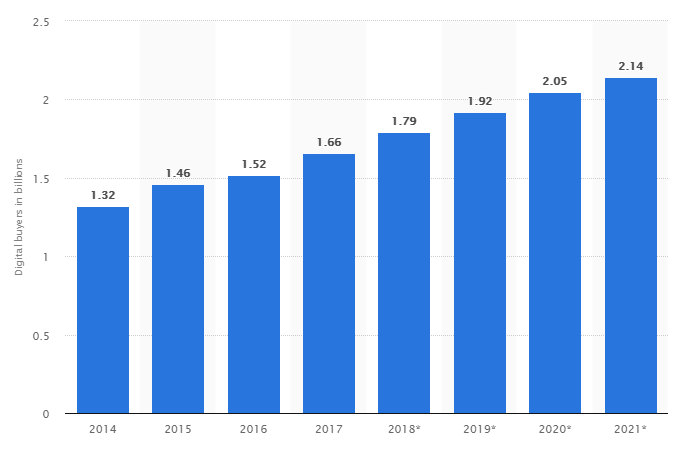
\includegraphics[width=\linewidth]{img/global_buyers_2017.png}
  \caption[]{The total number of digital buyers by year, in the 2014-2021 interval \footnotemark[1] \footnotemark[2]}
  \label{fig:global_buyers_2017}
\end{figure}

\footnotetext[1]{The numbers for the 2018-2021 interval are estimates based on the actual data}
\footnotetext[2]{Image from \cite{global_buyers_2017}}

\begin{figure}[ht]
  \centering
  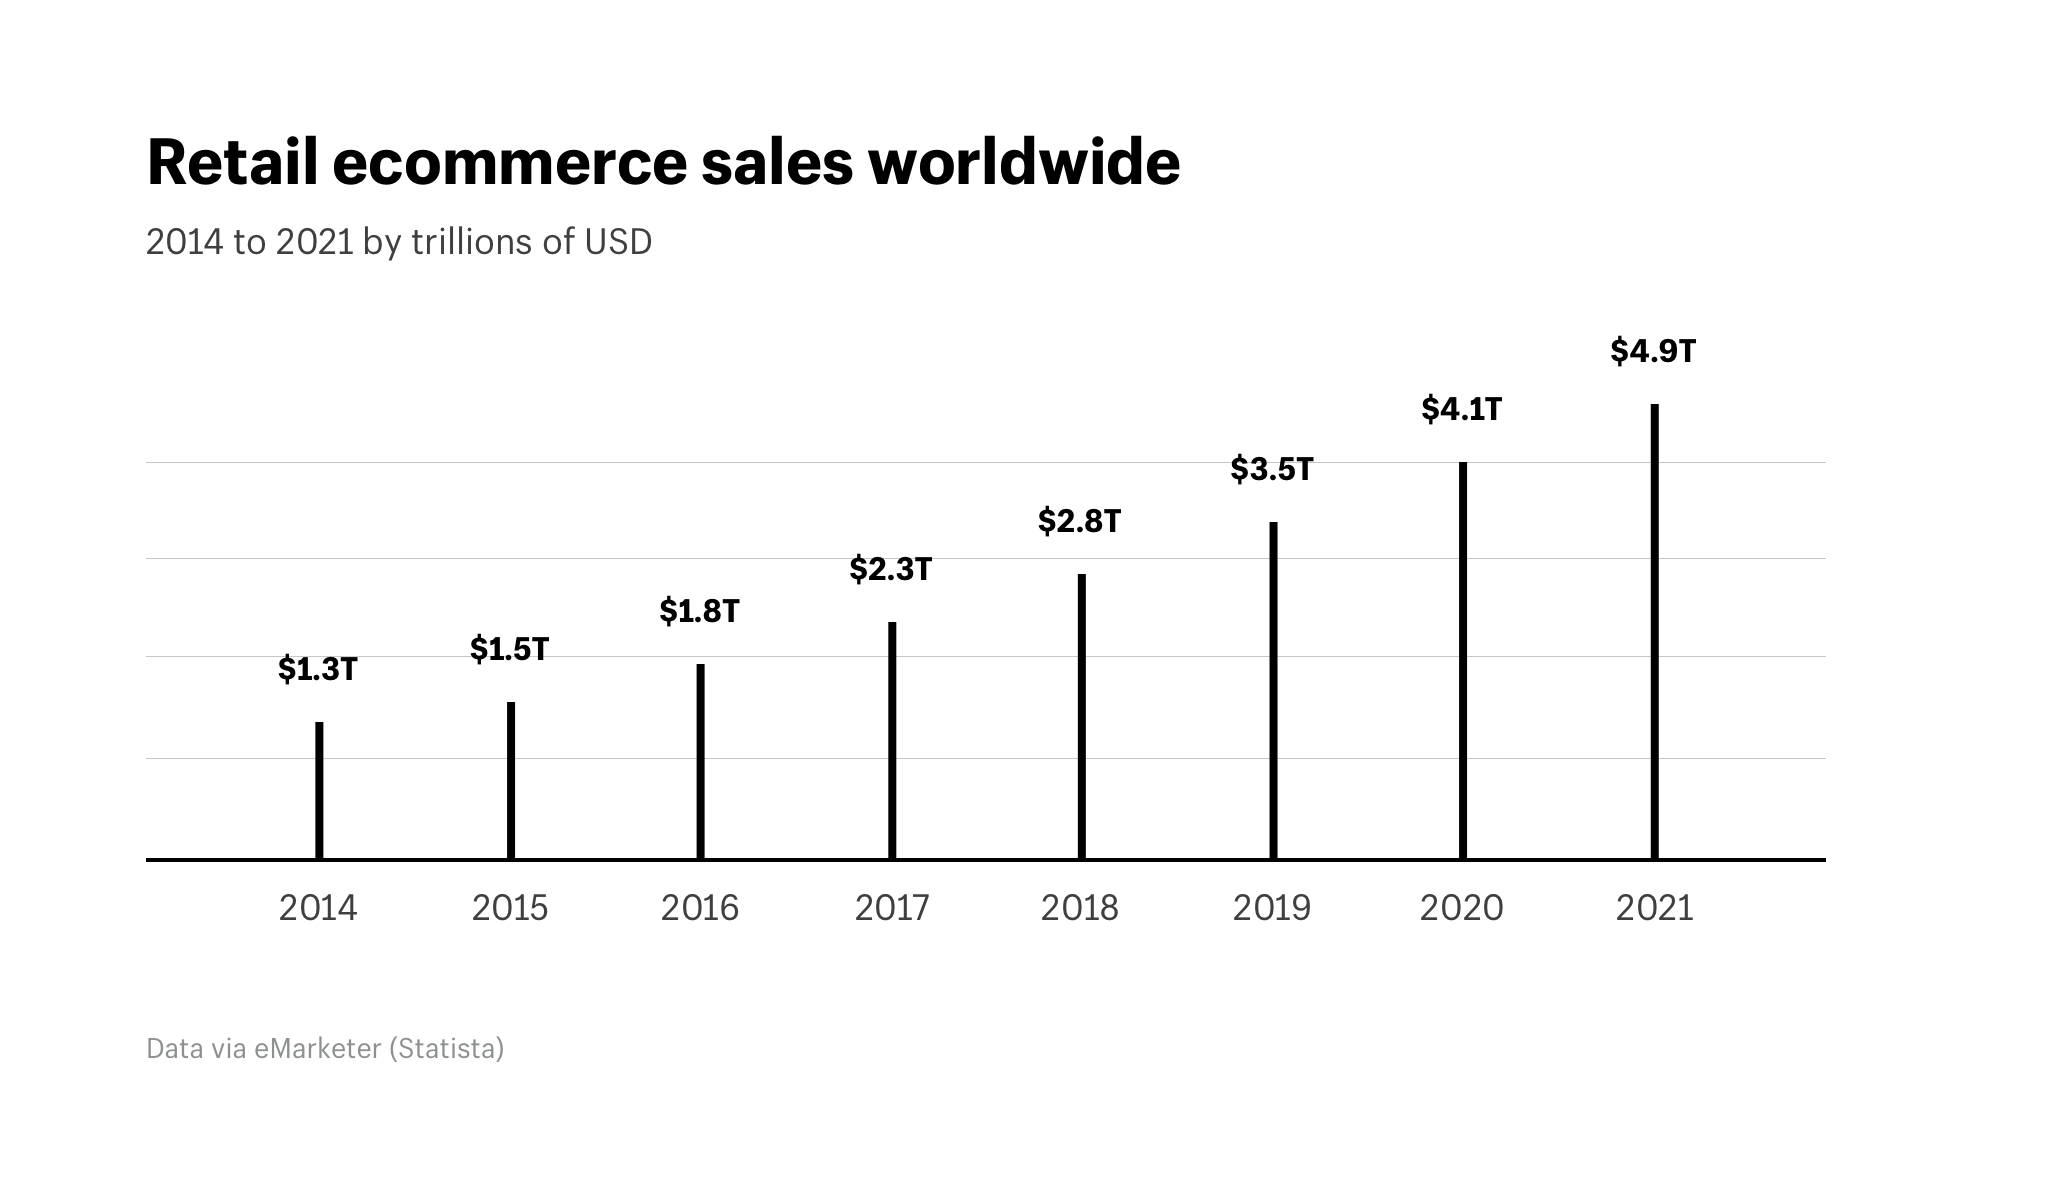
\includegraphics[width=\linewidth]{img/Retail_ecommerce_sales_worldwide.png}
  \caption[]{The total revenue generated by ecommerce sales by year, in the 2014-2021 interval \footnotemark[3]}
  \label{fig:global_revenue_2017}
\end{figure}

\footnotetext[3]{Image from \cite{global_revenue_2017_image}}

Humans as consumers, on the other side remained unchanged in two aspects which are relevant to our situation: one being that they will always try to seek the easiest way of doing a task and the other being the nature of constantly trying to spend less on the product they wish to buy. Unfortunately, from these perspectives the modern webshops can be a blessing as much as a burden. They allow you to purchase whatever you need and have it delivered to your doorstep with the minimal amound of physical work necessary. On the other hand they eliminate the option of good old bargaining, but given the vast number of retailers, prices are much more diverse also. And because of the fact that the customer can just as easily click a few times to buy a product from one retailer as from the other, the greatest way for a consumer to save money on their purchase is to find the retailer with the lowest price. As such, people who intend to save some money on their online purchases end up spending valuable amounts of time looking for a product in the webshops they know, which is a very limited number from the ocean of options they would have. These people usually end up just accepting the price they find in the first few webshops to reduce the time they spend shopping. What's more, some actually trustworthy webshops might not even have a very user-friendly interface, often confusing customers when they wish to purchase a product. This means that the probability of finding the lowest price is minimal and the process is extremely time consuming, inefficient and often tiring.

Online retailers, very similarly to their offline counterparts, have a major target in their activities too, that of reaching as many consumers as possible, and creating customers out of them. This, of course can be done via advertisements, but reaching a great amount of people with an advertisement placed on a high traffic website, such as a social network, can be extremely expensive nowadays. Taking into consideration another factor, such as the possible bad reputation the website on which the advertisement appears can also negatively impact the web retailer's or the product's image in the consumer's subconscious. The final, and probably greatest threat to the advertisement based attempts to reach customers is the usage of ad-blocking software, which modify accessed websites' DOM, completely eliminating elements containing advertisements. According to some studies regarding ad-blocking software usage \cite{adblock_stats}, 236 million desktop users actively used ad-blockig software in December 2016 and 2.3 million mobile users browsing the web from a browser that blocks advertisements by default, majorly due to the fact that 'too many ads are annoying or irrelevant'. This means that many users wont even get to see the advertisement the retailer is paying for, and even if they do, it's highly probable that it is of such poor quality or so invasive that the user will just get annoyed by it and he will develop a kind of hate for it.


\chapter{Project Objectives and Specifications}

\section{Introduction}

The purpose of this chapter is to collect, analyze, and define high-level needs and features of this license thesis. It focuses on the capabilities needed by the stakeholders and the target users, and why these needs exist.


\section{Positioning}
\subsection{Problem Statement}

Everyday more and more people are using the internet to buy what they need, from car tires to shoes, from a mobile phone to groceries. Due to the fact that the number of people shopping online increased thus increasing the demand for these opportunities, a naturally companies increased the supply by each creating one or more webshops offering the same product at different prices. This leads to the clients being lost among the options that have, and in a world where you would want to save money at every spending, a tool is necessary for the everyday webshopper to find the best price for their preferred product.

\newcolumntype{g}{>{\columncolor{lightgray}} m{0.45\linewidth}}

\begin{table}[H]
  \centering
  \begin{tabular}{| g | m{0.45\linewidth} |}
    \hline
    \textbf{The problem of}                 & looking for the cheapest offer for a product a client wishes to buy         \\
    \hline
    \textbf{affects}                        & everyday people doing their shopping online                                 \\
    \hline
    \textbf{the impact of which is}         & excessive time spent looking for an offer, ending in unsatisfactory results \\
    \hline
    \textbf{a successful solution would be} &
    easy to use
    easily accessible
    able to track the prices of a set of products across multiple webshops
    easy to extend to cover other webshops
    \\
    \hline
  \end{tabular}
  \label{table:problem_statement}
\end{table}


\subsection{Product Position Statement}

The Financial Efficiency Boosting System (FEBS) comes as a solution to the problem presented in the previous section by the use of web crawling, a web platform and a Google Chrome extension.

\begin{table}[H]
  \centering
  \begin{tabular}{| g | m{0.45\linewidth} |}
    \hline
    \textbf{For}              & customers of webshops                                                                                           \\
    \hline
    \textbf{who}              & need a tool to simplify their search for a good price                                                           \\
    \hline
    \textbf{The FEBS}         & is a system which tracks a set of products on online marketplaces                                               \\
    \hline
    \textbf{that}             & stores current data about products and tells the user about the lowest price of the product they are looking at \\
    \hline
    \textbf{unlike}           & compari.ro                                                                                                      \\
    \hline
    \textbf{The FEBS will be} &
    more accessible

    easier to use

    more intuitive                                                                                                                              \\
    \hline
  \end{tabular}
  \label{table:product_position_statement}
\end{table}


\section{Stakeholder and User Descriptions}
\subsection{Stakeholder Summary}

\begin{table}[H]
  \centering
  \begin{tabular}{| m{0.3\linewidth} | m{0.3\linewidth} | m{0.3\linewidth} |}
    \hline
    \rowcolor{lightgray} Name & Description                                                       & Responsibilities                                                       \\
    \hline
    \textbf{Webshop customer} & Person who engages in online shopping                             & Find the product they wish to buy and/or track                         \\
    \hline
    \textbf{Online merchant}  & Retailers of products who have their products tracked in the FEBS & Have the data about their products as clear and accessible as possible \\
    \hline
    \textbf{FEBS developer}   & Person who creates and maintains the FEBS                         & Create, improve and offer technical support for the FEBS               \\
    \hline
  \end{tabular}
  \label{table:stakeholder_summary}
\end{table}


\subsection{User Summary}

\begin{table}[H]
  \centering
  \begin{tabular}{| m{0.22\linewidth} | m{0.22\linewidth} | m{0.22\linewidth} | m{0.22\linewidth} |}
    \hline
    \rowcolor{lightgray} Name      & Description                                      & Responsibilities                                                                      & Stakeholder      \\
    \hline
    \textbf{Unregistered customer} & Person who rarely engages in online shopping     & Access the application to find a good offer                                           & Webshop customer \\
    \hline
    \textbf{Registered customer}   & Person who frequently engages in online shopping & Access the application to find a good offer and add products to their favourites list & Webshop customer \\
    \hline
  \end{tabular}
  \label{table:user_summary}
\end{table}


\subsection{User Environment}
\subsubsection{Users}

The application is public and the number of users may fluctuate based on the time of the day/week/month/year. The total number of supported users depends on the server.


\subsubsection{Time Limits}

The application should be available all the time, except for maintenance downtimes or unpredictable/uncontrollable downtimes such as power outages. A user can use the application anywhere from a minute if he finds an ideal price to a large time period if they wish to add a product to their favourites list to have it in an easily accessible location.


\subsubsection{Collaboration}

The application is used by a single person, anything a user performs with the system should not influence other users’ experience.


\subsubsection{Infrastructure}

The application will be accessible from web browsers. For full functionality a desktop based Google Chrome will be necessary, as this is the only browser to which an extension will be developed for further ease of use.


\subsection{Summary of Key Stakeholder or User Needs}

\begin{table}[H]
  \centering
  \begin{tabular}{| m{0.18\linewidth} | m{0.08\linewidth} | m{0.18\linewidth} | m{0.26\linewidth} | m{0.21\linewidth} | }
    \hline
    \rowcolor{lightgray} Need                     & Priority & Concerns             & Current solution         & Proposed solution                                        \\
    \hline
    \textbf{Support a multitude of domains}       & 0        & Customers, Merchants & Crawler for each domain  & Analyze and implement a crawler for each new domain      \\
    \hline
    \textbf{Easy to use interface}                & 1        & Customers            & Web platform             & Google Chrome extension which recognizes its environment \\
    \hline
    \textbf{Have an up to date database of items} & 1        & Customers, Merchants & Crawlers for each domain & Run the crawling task at regular intervals               \\
    \hline
  \end{tabular}
  \label{table:summary_of_key_stakeholder_or_user_needs}
\end{table}


\subsection{Alternatives and Competition}

There are similar tools currently available. One of those is compari.ro, which also lists the different webshops and prices for an item, but the fact that a client would have to actually access the website technically makes it harder to use than accessing a Google Chrome extension that is always present and provides data at one click distance.


\section{Product Overview}

The Financial Efficiency Boosting System should provide an easy to use way to users to see the best offer for their desired product. This concept can be seen in figure \ref{fig:app_system_diagram}.

\begin{figure}[H]
  \centering
  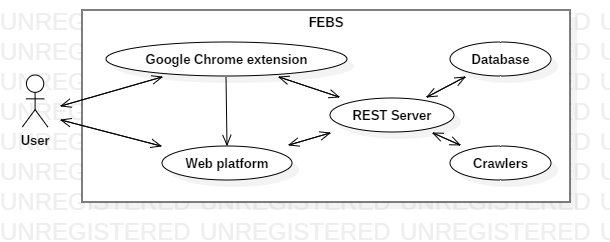
\includegraphics[width=\linewidth]{img/app_system_diagram.png}
  \caption{The FEBS's system diagram}
  \label{fig:app_system_diagram}
\end{figure}


\subsection{Product Perspective}

Compared to some competitors, such as compari.ro or PriceMon, FEBS aims to further ease the interaction of the user with the system by offering a font-end through a Google Chrome extension.
FEBS is a standalone application thus it is not part of a larger system.


\subsection{Assumptions and Dependencies}

A client is assumed to have a constant internet connection while using the application.

For the server side:

\begin{table}[H]
  \centering
  \begin{tabular}{| m{0.2\linewidth} | m{0.7\linewidth} |}
    \hline
    Database                     & \textbf{MySQL}                                                                                                              \\
    \hline
    Programming language support & \textbf{Java 8}, \textbf{Python 3}, \textbf{Angular 7}                                                                      \\
    \hline
    Frameworks, packages         & for Java: \textbf{Spring framework 2.1.3} or larger, \textbf{MySQL connector 8.0.13}, \textbf{Commons codec 1.12} or larger

    for Python: \textbf{Scrapy 1.6.0} or larger, \textbf{requests 2.22.0} or larger

    for Angular: \textbf{Angular CLI 7.2.4}                                                                                                                    \\
    \hline
    Miscellaneous                & \textbf{Node.js}, \textbf{Node Package Manager (NPM)}                                                                       \\
    \hline
  \end{tabular}
\end{table}

For the client side:

\begin{table}[H]
  \centering
  \begin{tabular}{| m{0.2\linewidth} | m{0.7\linewidth} |}
    \hline
    Web browser & \textbf{Google Chrome 75.0.3770.100} \\
    \hline
  \end{tabular}
\end{table}


\section{Product Features}

\begin{enumerate}
  \item \textbf{Simplistic web platform}

        The web platform should be as simple as possible so that the user can use and navigate it with maximum ease, while still offering the necessary features to accomplish the necessary.

  \item \textbf{Context recognition}

        The Google Chrome extension should automatically check if the user opens a link to a supported domain, in which case it automatically activates in case the user accessed the URL of a supported product it can shows different things if the webshop sells the product at the cheapest price or not: a message stating that the user is looking at the best offer or a link to the product page of the webshop with the cheapest price.
\newpage
  \item \textbf{Data monitoring}

        The system tracks changes about the supported products and refreshes the already available information and each distinct running of the respective crawlers.
\end{enumerate}


\section{Other Product Requirements}

\begin{enumerate}
  \item \textbf{Visually minimalist interface}

        The front-end of the application should be as clutter-free as possible, thus improving intuitiveness and ease of use.

  \item \textbf{Usability}

        The application should require close to no input from the user, as it should recognize its working environment to automatically help the user find the cheapest offer. In case user input is necessary, it should be as intuitive as possible to do this, such as interacting with a search bar on the web platform.

  \item \textbf{Performance}

        The system’s performance is measured in the client side response time, which should be at most 5 seconds for most operations.

  \item \textbf{Availability}

        Besides maintenance downtimes, which should take at most 2 hours each week, preferably in a time period when there is as little user activity as possible, there shouldn’t be any availability issue.

  \item \textbf{Scalability}

        The application should be able to serve many concurrent users without introducing too much stress on the system.

  \item \textbf{Maintainability}

        The system should be easily maintained, as most problems could be solved by either rebooting one of the services, or fixing an outdated web crawler.

  \item \textbf{Extensibility}

        The application should be easily extensible by adding supported products, adding URLs from supported domains to the existing products to gather data about them, or create further crawlers to support more domains.

\end{enumerate}


\chapter{Bibliographic Research}

The project's main scope includes the price and information tracking of certain products and by accomplishing this, web scraping becomes the main element in the application. During the bibliographic study part of this project's elaboration I read scientific articles, books and papers to learn about other people's attempts in accomplishing similar tasks and about possible algorithms and methods of going about it. In the following sections I will present the information learned from these materials.

The Financial Efficiency Boosting System heavily relies on web scraping to keep its data up to date. Web scraping is done using small, automated programs called web scrapers or spiders. Web scraping can be said to differ from web crawling by the purpose and task of its spiders. Crawlers are generally spiders used by search engines to index websites by downloading HTML pages through sending HTTP requests to URLs, parsing the page to extract further URLs and following extracted links. Usually, the bots which are used to download responses (not only HTML) from a web site by sending requests to certain URLs and extracting unstructured data for storage, analysis or manipulation are called scrapers. To summarize: crawlers are used for exclusive URL extraction and scrapers are used to extract any kind of data from the responses of a server.

In article \cite{crawlers_paper1}, the authors define some types of crawlers: Breadth First Crawler, Incremental Web Crawler, Form Focused Crawler, Focused Crawler, Hidden Web Crawler, Parallel Crawler, and Distributed Web Crawler.

The Breadth First Crawler starts with a tiny collection of URLs and then explores other pages basically through breadth-first fashion, but often prioritizing pages based on their importance. This approach is not necessary for my project, since I don't require the crawlers to access any further links for data extraction, as the necessary data can be found on the start pages.

The Incremental Web Crawlers are designed for continuous execution, applying pre-defined crawling cycles during their running. Doing crawling based on this category involves some changes to the basic concept of execution of a crawler. Because non-incremental crawlers are not designed to always run, they don't store the state of a web page for some further use and thus they download it every time the crawler is called. Incremental crawlers on the other hand would suffer a major perfomance penalty if they would just download and crawl every webpage continuously. For this, data from previous crawls is used through an adaptive model to select the pages which should be updated. This grants the data extracted by this type of crawler increased freshness and enables a lower system load. This solution introduces some amazing conepts which would help for larger, industrial sized projects, but is overly difficult and overshoots the scope of this project.

Form Focused Crawlers handle web forms. Form Crawlers incread performance by not accessing useless paths. This is done by learning facts about web pages, limiting the search of pages to a specific topic and integrating adequate crawl-stopping features. Pages and links are classified based on an algorithm and they are then stored in a database for future use. This is not necessary for my project as there shouldn't be a long crawling path, as search engines would need, only the starting URLs should suffice.

Focused Crawlers are based on a hypertext classifier developed by S. Chakrabarti in 1999, further described in 2003 in his book, titled "Mining the Web". This type of crawler relies on three components: a classifier for crawled page relevance based on which a decision is taken for further link exploration, a distiller which determines how central a web page is to set its priority, and the main element is the crawler which has a dynamically controllable priority, handled by the presented classifier and distiller. The focused crawler fixes the problem of uselessly crawling pages which have a minor relation to the topic in which the crawling process is run. This is done by searching to a given priority depth from a highly related web page. This solution regards deep URL exploration, which is not present in my project, so it is irrelevant.

Hidden Web Crawlers aim to solve the greatest limitation of crawlers, that of being able to only crawl the Publicly Indexable Web (PIW). A large amount of useful data is found in databases which is not exposed to the PIW. The area where they can be found is called the 'hidden web' or 'deep web'. Publicly indexable web pages are those which are accessible by ignoring search pages and forms which require authorization or prior registration, aka those pages which do not require any specific human interaction. Hidden Web Crawlers interface with private APIs to retrieve data present on the 'hidden web'. This method, though useful, usually requires extensive negociations with the companies owning the APIs which are to be used, thus being immensely time and money consuming, not even mentioning the fact that not anybody could reach the point of negociations. Hidden Web Crawlers immensely overshoot the scope of this project and will not be used.

Parallel Crawlers increase crawling performance and decrease the time necessary for running crawling tasks by spawning parallel processes for performing crawling tasks on multiple URLs at the same time. This is highly beneficial, as due to the web's size, usually a crawling task runs on multiple URLs, sometimes going into the number of thousands, millions or even billions in some cases, and running them on a single process could end up taking days, weeks or even months, depending on the depth and complexity of the task. This feature is very useful and will be used in the project.

Distributed Web Crawlers are similar to the Parallel Crawlers, as in they aim to solve the issue of having to handle a large amount of web pages by running it in parallel processes. In the case of Distributed Web Crawlers, this is achieved by the following process: URLs are distributed by a server to several crawlers, which then retrieve and process the web pages in parallel. The extracted data is sent into a central module, which, since the paper focuses on indexing crawlers, is a central indexer, which then returns the URLs back into the crawl-indexing cycle to the crawlers. The exact example described in the paper is useless for my project since I don't aim to execute an indexing task with my crawlers. Adapted to my case though, it has parts which are useful for me, such as distributing the crawling task and then uniting the results in a single module, which in my case should be the database.

According to the information present in \cite{crawlers_paper1}, a good web crawler should have some basic features. These features will be desribed in the next paragraphs.

Speed is one of the vital properties a crawler should posess, as, according to the information in the paper mentioned, almost 90 thousand pages are fetched a day by a simple crawler,which would lead it to fetch a small number of 1 million pages would take 11 days, 10 million getting to half a year. Achieving speed in the crawling process can be greatly helped by increasing the level of parallelization of the crawling process.

The property of politeness refers to the crawling system's method of sending requests to the server. A system that sends requests at some delay to decrease the load on the server is called polite. Politeness is important for a crawling system from two perspectives. Firstly, a huge sudden load might very easily crash a server, thus making it impossible to send the other requests or get a response from the server, thus failing the crawling task. Another aspect is that nowadays many servers have anti-crawling mechanisms implemented that detect very rapid or regular requests, and then they block the IP from where the requests originated. This possibly fails the running crawling task and makes the running of future tasks impossible.

Respecting excluded content is done by respecting a web sites 'robots.txt' file. This file describes the behavior of crawlers. The file must be fetched and read ahead of doing any further crawling work and the crawling process must be adapted to the rules in it. Not respecting these rules can lead to the crawler's IP being blocked, thus failing the crawling task and making running future crawling tasks impossible.

A good crawler should be able to detect duplicated data and decide to not use it. This is necessary to reduce the amount of redundant tasks in a crawling system, boosting performace of certain parts.

For indexing purposes, there are two more necessary things a crawler should conform to. Firstly, ontinuous crawling is advised, as regular, full crawling tasks are ineficient. Secondly, they should be able to detect spam links, such as advertisements and not extract them. This situation is not our case though, so these constraints do not apply to my project.


\section{Similar applications}

In this section I will explain some applications or projects which I found to be accomplishing a similar task to the application I proposed to develop.


\subsection{Effective Web Scraping with OXPath}

In their paper \cite{oxpath_scraping} Giovanni Grasso, Tim Furche and Christian Schallhart describe a web scraping solution using the OXPath wrapping language, designed and developed by them.

The authors call OXPath a "wrapping language that is nevertheless expressive and versatile enough for a wide range of scraping tasks". In their paper, the authors wish to introduce the 'declarative navigation' paradigm of web scraping. The authors state that there is an observable lack of stock tools or frameworks for software developers to use, stating that the available crawling solutions are often using a large stack of complicated tools. The authors reacted to this universal fact by developing OXPath to offer developers a lightweight tool for web scraping.

On OXPath's repository page \cite{oxpath_repo}, we can find out that OXPath is defined as an XPath extension for web data extraction with additional Actions (click, form filling), Extraction Markers (qualifier for nodes to be marked as a representative for records), Style Axis and Visible Field (a method of allowing users to select nodes based on any CSS attribute), and Intensional Axes (a method of selecting nodes through multiple conditions).

OXPath has been used in several applications since its development. One of these applications is 'DIADEM', developed at Oxford University on unsupervised domain-specific web object extraction. Its aim is to convert unstructured internet information into organized data without human oversight. OXPath is the chosen language forthe wrappers in DIADEM becuase they can be run with great performance and low cost. DEQA is a project at Leipzig University which aims to create a full answer providing system for the deep web, where the web sites are plain HTML for security purposes. In this project OXPath is tasked with creating structured data from the websites. Arcomem is an European project aiming to create community memories from digital archives, mostly developed in France. Basically, this project takes blogs, web forums and social networks, takes un-duplicated data from posts and archives them. In this application OXPath fulfills three purposes. Firstly, it detects the type of web app, then it retrieves all the originally hidden content by navigaing on links such as 'show all comments', and finally, it extracts the data from the resulting page.

Unfortunately, OXPath is too low level, badly documented and lacking tutorials, so it will not be used for my project. It's worth mentioning that it is a respectable language which seems to have a future in the web crawling domain in the future.


\subsection{Monitoring Product Sales in Darknet Shops}

York Yannikos, Annika Schäfer and Martin Steinebach describe a darknet crawling solution for monitoring sales in their paper \cite{darknet_crawling}. This solution seems to combine the 'Hidden Web Crawlers' and 'Parallel Crawlers' type of crawlers from the paper \cite{crawlers_paper1} presented at the beginning of the chapter. Even though the darknet and accessing it is out of the scope of this project, I found the topic interesting, and their solution exceptional. There also is a major difference in the task accomplished, in that they were monitoring product sales for further analysis and I track product prices for users' utility. It is worth noting that the marketplaces on the darknet and the transactions happening there are far from the scope of ordinary ecommerce transactions and may sometimes even face the user with facts about our world which may leave the curious but faint of heart scarred. Ecommerce on the darknet is done using bitcoin based transactions.

The darknet represents the non-indexable part of the internet. It is accessed via the Tor browser, which relays and encripts requests and responses through three series of IP addresses, thus creating a layer of protection, similarly to how a VPN service operates. This works using the 'Onion Router', which sends the network traffic through a series of nodes where the information is encrypted using an assymetric encryption algorithm, thus piling up the encryption layers, similarly to an onion. The Tor browser is designed with privacy, anonimity and freedom in mind: besides its VPN-like way of handling requests, it also has a special security setting, which can disable JavaScript on web pages to eliminate its tracking tools. The Tor browser has compiled a list of advices that the user should conform to to maintain a maximal level of anonimity. The Tor browser also allows the hosting of hidden services which can only be accessed using the browser. While ordinary websites outside Tor can be easily accessed by changing the website's hostname to its respective IP address, that does not work for Tor's hidden services. Hidden services use a special '.onion' top-level domain name and a hostname that can not be resolved through DNS, instead is constructed from the host's public key. This means that accessing such services only work using the Tor browser.

The implemented technique heavily relies on regular crawling techniques, except that they needed to add support to the SOCKS proxy. They contacted several darknet ecommerce vendors asking for bitcoin addresses. These addresses were used to continuously monitor the bitcoin transactions of the vendors which provided them. This was done via a client they implemented for the BlockTrail API. Unfortunately BlockTrail has since been terminated. The tracking was used in correlation with scrapers to track sales of different vendors, their products and the changes they made. They ran a test crawling process for a week, running the crawlers three times a day, and afterwards, for actual data collection they ran the crawling process similarly, but for 14 weeks. The extracted data was then used to make a study about the categories of products, number of transactions, and transaction values.

This study has provided me with insight into the differences to the crawling process between regular, World Wide Web based crawling and darknet crawling. Since my project does not deal with the darknet, unfortunately nothing was usable from this paper.


\subsection{The Use of Web Scraping in Computer Parts and Assembly Price Comparison}

Leo Rizky Julian and Friska Natalia talk about using web scraping to create an application which recomends its user an ideal computer build in their paper \cite{pc_build_tracker}. They go on to explain how a casual user would go about trying to find the best offer for buying certain components. They say that, generally, a customer would not only want to buy any cheapest product but also have a balance between cheapness and quality. 

Julian and Natalia go about describing the process they took for scraping the 5 websites they chose for the project by stating that they used the Pentaho software to extract the necessary data data. This conforms with the concept stated in their paper \cite{oxpath_scraping} by Grasso, Furche and Schallhart, which holds that, in the scraping domain, the availability and use of low level APIs are rare, and that high level, complex applications dominate this market section. Getting back to the process Julian and Natalia took to extract useful data from their website, they describe how they split this section of their task into multiple parts. Firstly, they described the process of finding the patterns in the HTML structure of the websites that precisely locate the data they needed. They noted how this step strictly consisted of analyzing the HTML and trying to find the tags to introduce in the Pentaho software to extract the data. The second part of their process consisted in extracting the data using the Pentaho software and the tags they located in the first step. They continue to describe how the data returned from the data extraction step is still quite noisy and in need of cleansing and transformation. For this step they, again, used the Pentaho Data Integration software. They go on to explaining how the data was cleansed by separating the useful information from the extra data that the extraction step returned. The data they needed was the names, prices and categories of computer parts. HTML files might often have a structure that does not allow the pinpointing of certain elements, such as tables, where the rows do not have special tags marking the data represented in them. This leads to the extraction phase extracting the whole table, which then needs to be separately parsed and data needs to be selected from it. Other common types of impurities might include pre- or post-trailing spaces or data being mashed together under one tag, when they should be separated. The extracted and cleanssed data was then introduced into a Microsoft Excel document for storage. I think this method is a bit primitive, but I can see how this solution fits their purpose.

The authors have used a waterfall approach during the elaboration of the project. For designing the application, Julian and Natalia have used the Unifid Modeling Language (UML) diagrams for documenting the application's requirements. For the implementation phase of their application Julian and Natalia grouped the tasks into two groups: data acquisition and the development of a web application. For data acquisition they furter distinguished some steps. They first used Pentaho to grab URLs and categories of computer parts. The resulting data was put into 'cube' files, which were then used in the next step. The following step was to use the fetch the HTML of the web page using HTTP requests sent to the component's URL. In the HTML file the authors then found some patterns based on the classes or attributes of HTML nodes to extract the required data. In the second step of their data acquisition section is cleansing the extracted data, done using regular expressions. The cleansed data is then introduced in a Microsoft Excel spreadsheet. In the third step the authors sorted the data from the spreadsheet based on the product name to group data belonging to the same product and introduced the resulting data into a database. As part of their implementation, the authors created a matching table that matches the names of the components present on the websites to the actual name of the component, the one they use to indentify them. The final result of their project was a web app that compared prices of computer parts from five different web sites, simulated PC assembly, and recommended PC builds based on three categories: personal home computer, business computer or gaming computer.

The project elaborated by Julian and Natalia was a very useful starting point, as it detailed some key aspects of web scraping that need to be followed for successful data extraction. Unfortunately, since they used an external software tool to execute the data scraping part of their application, this was not very useful for me, since I aim to implement my own scrapers.


\chapter{Analysis and Theoretical Foundation}

\section{RESTful Web Services}

The concept of Representational State Transfer (REST) as an architectural style for distributed systems was invented and presented in 2000 by Roy Thomas Fielding in the 5th chapter of his doctoral dissertation \cite{fielding_rest_definition}. Fielding described it as follows: "REST provides a set of architectural constraints that, when applied as a whole, emphasizes scalability of component interactions, generality of interfaces, independent deployment of components, and intermediary components to reduce interaction latency, enforce security, and encapsulate legacy systems".

Fielding build the REST style as a hybrid style, including constraints from other, already defined architectural styles. REST was conceived from the ground up, starting with the client-server architecture, adding several constraints: statelessness, caching, a requirement for uniform interface, a layered system, and code-on-demand. The client-server architecture was used as a first step in bulding the architectural style. This was necessary in order to divide the user interface from the data storage, thus portability and scalability was improved. Adding statelessness made it mandatory that all the information necessary for the server to fulfill the request to be included in it. This means that all the information regarding the session has to be stored on the client. Statelessness is a compromise between reliability, scalability and visibility, at the downside of a potential hit in network performance due to more and more repetitive data being sent in a sequence of requests. Fortunately networking technology advanced from the, back then state of the art twisted-pair copper telephone wire solution using ADSL to provide speeds of 10 Mbit/s with 56 kbit/s download speeds being more common, while today's optic fiber solution is using the G.fast protocol to reach 1 Gbit/s speeds \cite{historical_net_speeds}, so the presented disadvantage of statelessness shouldn't be an issue nowadays. The option of caching response data was added to improve network efficiency. This means that whenever a response is sent, data should be labeled as cacheable or non-cacheable. In case a response is cacheable, a client may store and reuse the data for other equivalent requests. This allows some interactions to be eliminated, scalability and efficiency to be improved. The downside introduced with caching is that cached memory can reduce reliability due to stale data being reused. The main introduced aspect was an emphasis on making the interface between components uniform. Adding the concept of generality to the component interface simplifies the system architecture, improves the visibility of interactions and dissolves coupling between implementation and provided service, which in turn allows independent evolution of the two. The trade-off lies in decreased efficiency due to the data being passed in a standard form, rather than one tailored to the application's needs. Interface uniformization is achieved through the application of four constraints: resource identification in requests, representation based manipulation of resources, the usage of hypermedia as a means of keeping the application state and self-descriptive messages. The concept of a layered system was introduced to protect and encapsulate services, creating a downside by adding some latency to the processing of data. Finally, code-on-demand was introduced to decrease the complexity of the client.

Web services that take advantage of the REST architectural style are called RESTful web services. These kind of web services grant compatibitlity between software systems. By using RESTful web services, client systems are capable of accessing and managing web resources by using a uniform and pre-defined collection of stateless operations. Web resources are defined as documents or files identified by their Uniform Resource Identifiers (URI), and accessed using their Uniform Resource Locators (URL). RESTful web services nowadays access web resources which are exposed an a URL form. The most commonly used way to communicate with a web service is via the Hypertext Transfer Protocol (HTTP). Systems can use the URLs to send HTTP requests to the web service, which then return an HTTP response with an error message, in case something went wrong, or the data requested. The data can be the contents of a file or the result of a method. This whole process is quite similar to a RPC based web service, but it's a less rigid solution than, for example, a SOAP based solution, which responds to specific method names \cite{resftul_web_services}. Thus, RESTful web services profit of the code-on-demand feature of the architecture while also keeping coupling to a minimum. The most common formats for representing data in an HTTP request or response is HTML, JSON or XML.


\subsection{The Spring Framework}
Spring is an application framework developed by Pivotal Software for Java, first released in 2002. It has several modules, providing a great number of services, the most important ones for me being the data access module, the inversion of control feature and the model-view-controller module.

Inversion of control (IoC) is a software engineering principle, falling into the architectual design patterns category, regarding the flow of control of the code. This principle inverts traditional flow, giving full control of execution to the used libraries, decoupling elements, increasing modularity and enabling extensibility. The concept of IoC is tightly related to the priciple of Dependency Injection. The Spring framework takes advantage of this pattern by integrating them. Dependency Injection is the standard way of linking components in the framework.

The data access module connects relational database management systems with the application using the spring framework. This is done using the Java Database Connectivity API (JDBC) and object-relational mapping tools, such as Hibernate ORM. Spring uses Hibernate ORM to map plain old Java objects (POJO) to data which is supported by databases such as the MySQL relational database management system. Hibernate then further uses JDBC to connect with the database.

The most important feature of spring for my situation is the model-view-controller module, which, being a servlet and HTTP based framework, makes the creation of RESTful web services easier. The Spring MVC module is based on the architectural pattern with the same name, thus introducing the decoupling of the model, view and controller from eachother. The model part of an application is the one that deals with the object modelling of the application's domain. This term encapsulates data management and logic. As part of the model-view-controller interaction cycle, it is responsible for receiving user input from the controller, executing it and sending updates to the view if necessary. The view part of the application is an independent user interface through which information from the model is exposed to the user. The controller of the application is the part which accepts the user input, validates it if necessary and passes it to the model as commands to be executed.

The Spring framework, uniting all its modules becomes an easy to use framework that greatly helps a software developer in building web applications with the Java EE (Enterprise Edition) platform. The lowest element of a Spring MVC based application are the entities. These are the classes which model the domain of the application. The Spring framework heavily relies on a set of annotations to mark certain properties or automatically generate beans from classes which can then be injected in other classes. Entity classes are no different, as have to be marked with the '@Entity' annotation before each class definition to be discovered by the framework. The attributes of these classes have to be annotated according to the position they will fulfill in the database. Based on these annotations and the attribute names Spring can automagically generate the complete database in the defined database management system, in such a way that the created database will be a prefect representation of the application model domain, supporting the data to be manipulated. The basic communication with the database is encapsulated in interfaces called 'Repository' and annotated with the '@Service' annotation so that they can be injected in the appropriate component in the business layer. These use the objects defined as 'Entities' and execute the SQL code that Hibernate generated based on the command given to it. After executing the SQL code, JDBC gets a value or set of values from the database and returns them further into the application, to the Hibernate session, which in turn converts it to the appropriate Entity object using ORM and returns it to the calling Repository. Classes encapsulating the business logic of the application also have to be annotated with the '@Service' annotation, so that they in turn can be injected into the 'Controller' classes. The direct interfacing with the rest of the application is done via the layer of 'Controller' classes, which are annotated with the '@RestController' annotation to mark their nature, and '@RequestMapping' annotation marking the path for finding the resources that are encapsulated in it and have further annotations to aid in locating them.

Using these mechanics and architecture, Spring becomes an ideal framework to use in the creation of a RESTful web service, which would then form the back-end of a full stack application.


\section{Web scraping}

A web crawler is a bot used to automatically explore web pages on the World Wide Web as a method of web indexing. A web scraper is a specific kind of web crawler, with the difference of it being used to extract data from the visited websites. The extracted data is usually persisted in a database for later analysis and/or manipulation. Web scraping is the act of using web scrapers in a system to extract some data from websites and then persist it in a database.

A web scraper operates on a set of simple steps. First, it receives a set of URLs usually called seeds to start scraping. The scraper sends an HTTP request to the URL to fetch the page, the response usually being in the form of HTML but in case the scraper has direct access to the application API, application data can be an option, which can be encoded in JSON or other formats. The received data then has to be parsed and preferably put into objects so that it gains a uniform structure. As a final step, the processed data should be stored in a database for further use. Scrapers may have a multitude of uses, such as data mining, online price monitoring and price comparison, contact scraping, weather monitoring and website change detection.

Web scraping is a very valuable tool in the modern world, seeing as the internet is filled with so much available and useful information publicly available. The development of the internet and the amount of content it holds has been much more rapid than that of web crawling solutions. As such, the domain of web crawling is still a field with major potential and space for major breakthroughs in fields such as text processing or artificial intelligence. Web scraping solution in use nowadays include manual copying, regex matching, HTTP request based scraping, HTML parsing, DOM parsing or computer vision based web scraping. The technique of manual copying involves a human agent manually opening a website on a browser, locating the necessary data on the webpage, copying it and then pasting it into a database. This method is extremely time and money consuming, as a bot does not need to perform physical actions and does not ask for a monthly salary. Unfortunately there are some cases where automated scrapers aren't able to do the job due to scraping blockers or lack of accuracy, therefore human labor becomes necessary. The regex matching technique involves taking the whole webpage in textual form and applying a regular expression based search on it to find the data necessary. This, again is quite inefficient and might even result in inaccuracies, because website HTMLs can be quite lengthy, finding the correct regular expression might take a very long time, and even be so long that it's would not be worth doing. HTTP request based scraping involves directly sending HTTP requests to a public API of the website we wish to crawl, thus having its resources exposed. This is by far the most efficient scraping method, as there is not too much hassle for the development team, as they don't have to bother with parsing the website in any way. Unfortunately there aren't too many websites freely exposing their API. HTML and DOM parsing are quite similar to eachother, because in the case of HTML parsing, the code is first converted into a DOM, and from there the technique is the same: the adequate elements are selected from it to narrow down the amount of text that has to be processed by other means. HTML parsing is the most commonly used attempt to web scraping. Computer vision based web scraping is a method which appeared as a response to the attempts to block other types of scraping bots on certain sites. Computer vision brings a more modern approach to scraping by combining machine learning with image processing to locate and extract data from a website. This web scraping method is much more computationally intensive than any other one before, therefore it cannot be used as a main approach to scraping.

There are several tools that could help in web scraping or pre-build web scrapers that already solve the problem. Wachete is a browser based tool for website change monitoring. Users have to include the URL of the page they wish to monitor with an option to then monitor its subpages up to three levels deep too. The step after giving a starting URL is selecting an area on the downloaded and presented page so that the tool can create a selector for it, setting the format of the data to be checked, and the frequency of the monitoring process. This means that the user is basically given a user friendly interface to create a scraper, which has every element necessary for a simple scraper: a starting URL, the crawling depth, the crawling frequency, and a single entry of data. cURL is a command line tool that can send requests to URLs, supporting a multitude of HTTP methods, as well as the inclusion of headers or cookies in the request. This makes it a decent tool to test the parameters of requests before implementing them in an actual scraper. Diffbot is a company which develops algorithms and APIs to extract information from a website based on machine learning and image processing. In the situation when a developer wishes to develop their own scrapers they would need extensive knowledge about HTTP requests, HTML, CSS, JavaScript and security elements such as session data. Fortunately there are frameworks specially designed for web scraping.


\subsection{Scrapy}

Scrapinghub, the developer and maintainer of Scrapy defines it as "an application framework for crawling web sites and extracting structured data which can be used for a wide range of useful applications, like data mining, information processing or historical archival." \cite{scrapy_docs}. It was first released in 2008 and is still in constant development, having reached the last major update, version 1.6 in January 2019. Scrapy presents itself as a quite complete and well documented web scraping solution. It includes several elements which are critical for web scraping: scrapers (called spiders) for data and link extraction, a powerful request making mechanism, both an XPath and a CSS based HTML selecting solution, a complete logging system, command line integration for generating projects and spiders, opening webpages for the developer to see how the framework sees them, or starting crawling tasks, amongst others.


\subsubsection{Scrapy Architecture} \label{scrapy_arch}

The Scrapy architecture is constructed from a few main elements. Understanding these components and the way they connect is vital for using Scrapy to its full potential An overview of the architecture and the data flow between its components can be seen in figure \ref{fig:scrapy_architecture}.

\begin{figure}[ht]
  \centering
  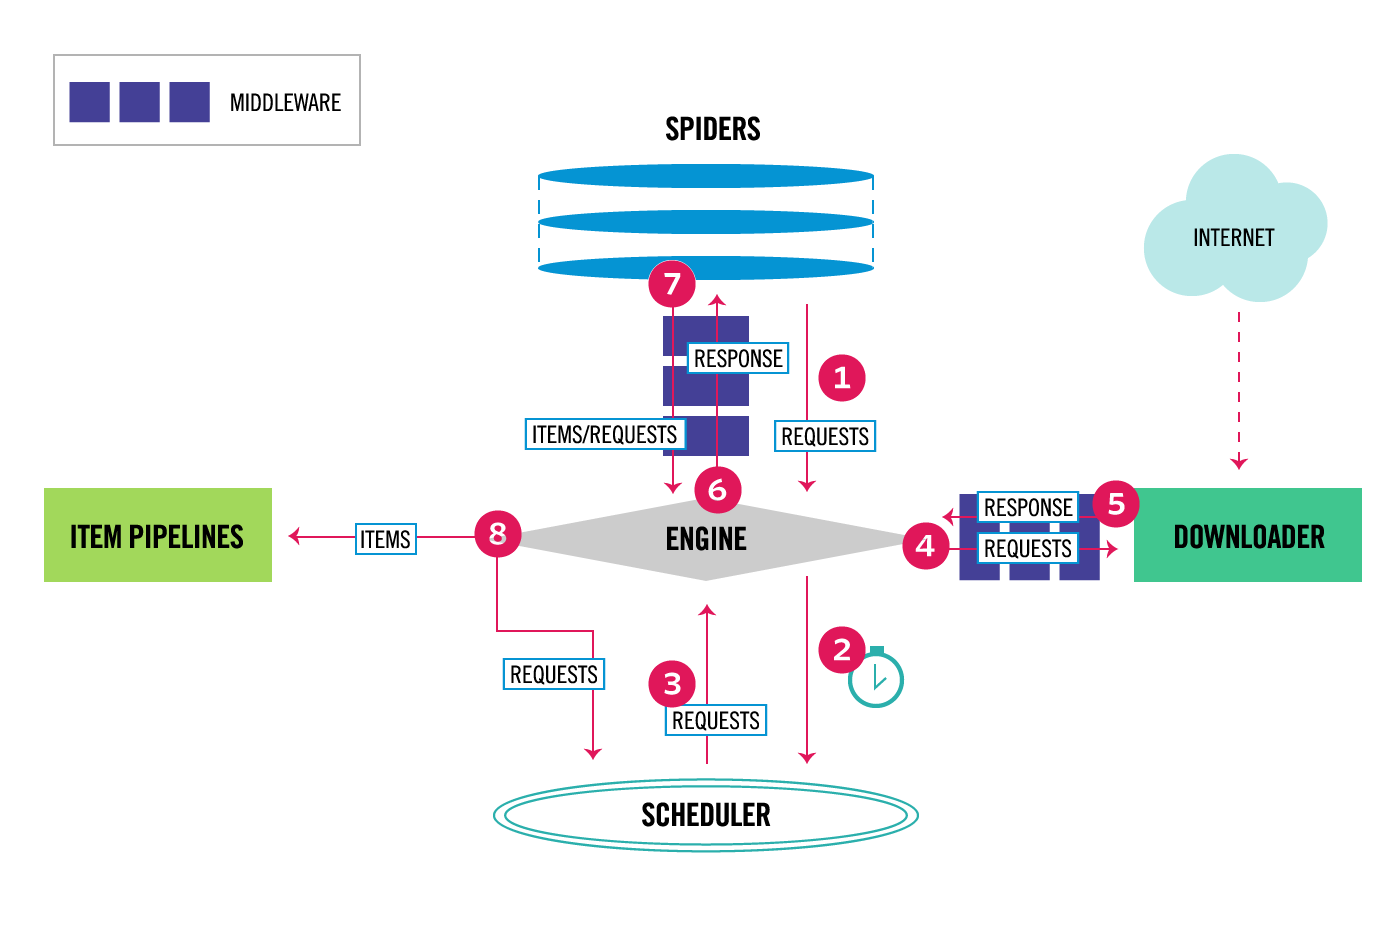
\includegraphics[width=\linewidth]{img/scrapy_architecture_02.png}
  \caption[]{Overview of the Scrapy architecture and data flow between its components \footnotemark[4]}
  \label{fig:scrapy_architecture}
\end{figure}

\footnotetext[4]{Image from \cite{scrapy_architecture}}

At the center of the architecture seems to be the Scrapy Engine, which controls the data flow between its elements, but actually the whole system revolves around the spiders. It is worth noting though that the Scrapy Engine is built on the Twisted event-driven framework. This means that the whole cycle is implemented using non-blocking code, granting concurrency to the applications written using Scrapy. Therefore writing blocking code while using Scrapy is contradictory to the whole idea behind this architectural decision \cite{learning_scrapy}. The whole scraping process starts with when a spider is invoked, either via the Scrapy command line interface or from a script. The spider then sends the details of the requests built based on the given start URLs, headers and cookies to the Engine. The Engine then passes these requests to the Scheduler adding a delay between the requests which are sent to the same website. The value of the delay is set by taking values set in the settings file of the project, or directly from the spider, if it has a \lstinline$download_delay$ attribute defined. If neither are defined, the delay takes a default value, which is 0. Setting a download delay might help with avoiding some scraping detection and blocking mechanisms which detect the interval of time and the regularity of the requests received from a given IP address. The Scheduler keeps returning requests to the Engine every time a previously sent request is completed, thus controlling the number of concurrent requests. The Engine forwards the recieved request from the Scheduler to the Downloader, which then fetches a response based on the given request and returns it to the Engine. This interaction between the Engine and the Downloader is done through a framework of hooks into the request/response handling. This part of the architecture is composed of elements called 'Downloader Middleware'. When activated, Downloader Middlewares alter the requests and responses passing through the Engine-Downloader section. Upon receiving them, the Engine in turn routes the responses to the spiders. The spiders then process the information contained in the request. One way of using Scrapy is extracting data using the built-in XPath and CSS selectors and inserting it into Items. Alternatively, additional requests can be created by using the spiders to extract URLs from the response similarly to how Item filling data is extracted. This second part of the iteraction between the Engine and the Spiders happens through elements called 'Spider Middleware'. They, similarly to the Downloader Middlewares, are a framework of hooks into the spider processing process. Spider Middlewares might seem to be useless at first, since the spiders should compeltely process everything. This might be true in theory, but there may be situations in practice where start requests, returned Items or extracted requests need post-processing, or some exceptions returned by the spider need to be handled. The extracted Items and generated requests are sent to the Scrapy Engine to be accordingly distributed: the requests generated from the URLs are sent to the Scheduler and the Items are sent to the Item Pipeline. The Item Pipeline is composed by a sequence of scripts that manipulate the returned item. They can be used to clean, validate and/or persist the data in the Items. The process repeats itself from the point where the Scheduler returns requests to the Engine until there are no requests left to process.


\subsubsection{Spiders}

A Web scraper which is generated by the Scrapy framework and run in the Scrapy cycle is called a 'Spider' according to scrapy. According to the regular definition of a web scraper, spiders take a list of starting URLs and at the end returns extracted data. Of course, in the background, the way this happens is more complex. Spiders form the core or the Scrapy cycle, as they create the requests to be sent and they process the response of those requests. Essentially, scraping couldn't exist without these spiders.

To be able to generate spiders, you should be inside the directory of a Scrapy project. Scrapy projects can be created using the \lstinline$scrapy startproject <project_name> [project_dir]$ command line command, which gets the project name as an argument, as well as the preferred directory for the project to be generated in, as an optional argument. Spiders can be generated using the Scrapy command line tool using the \lstinline$scrapy genspider [-t template] <name> <domain>$ command line command, which gets the spider's name and the web domain on which it should operate as arguments and as an optional argument, template, which is used to so that Scrapy can generate the spider from a list of predefined spider templates. If the 'template' optional argument isn't defined, it creates a blank spider in the 'spiders' directory of the currently open project. In case you are not in a project directory, the spider will be generated in the current directory, but this is not an ideal situation, since the spider can't run alone without a Scrapy environment and it will need to be moved to an adequate directory.

A generated spider implicitly includes some functionality and it automatically inherits the settings defined in the project unless explicitly defined otherwise. Implicit functionality may always be redefinied explicitly, thus overruling the minimal implicit definitions. One of the implicit methods is \lstinline$start_requests()$, which takes the \lstinline$start_urls$ and generates an iterable which includes the initial requests to be scheduled and performed. This iterable is then forwarded to the Scrapy Engine according to the description in subsubsection \ref{scrapy_arch}. When the spider receives the response to a request, one of two options can be executed: the callback method passed to the request is executed, or, in case no callback method was passed, the execution defaults to the \lstinline$parse()$ method, but essentially the all same the same purpose: parsing the response received to extract. Since the response is usually in the HTML format, parsing it most commonly consists in parsing the returned HTML. This can be done in two ways: with CSS selectors or with XPath expressions, by using the response object's \lstinline$.css()$ or \lstinline$.xpath()$ methods. XPath is a very powerful language which is used to select nodes in an XML documents, and it can be used in HTML aswell. It is worth noting that selecting elements using the CSS solution converts the selector to an XPath selector in the background, and applies this on the HTML to get the requested node. As thus, almost everything about the two object methods is equal after the CSS selector is transformed into an XPath selector. Both of them are implemented using 'parsel', a Python library created to extract data from HTML and XML using XPath and CSS selectors. Both of them return a \lstinline$SelectorList$ which can be used to further apply selectors to it, or data can be extracted via the \lstinline$.getall()$, \lstinline$.get()$, \lstinline$.re()$ or \lstinline$.(re_first)$. The \lstinline$.getall()$ method returns a list of extracted results, while \lstinline$.get()$ returns the first of that list regardless if it there are more or not. The regular expression based  methods are similar to the previously presented ones, except for the fact that they apply the regular expressions passed as parameters onto the selected result(s) and return either a list of unicode strings, in case of \lstinline$.re()$ or a single unicode string, which is the result of applying the regular expression to the first element in the \lstinline$SelectorList$, in case of \lstinline$.re_first()$. The resulting extracted data should be returned either as part of an Item or as the URL part of a \lstinline$Request$ element of an iterable containing the same type of elements. From this point onward it is either the Scheduler's job to continue with adding the returned Requests to the current list of incomplete requests, or some part of the Item Pipeline's job to manipulate the returned Item(s) in some way.


\subsubsection{Items}

Scrapy defines Items as "simple containers used to collect the scraped data." as part of their official documentation \cite{scrapy_docs}. Even though Scrapy spiders can return the extracted data in the format of Python dicts, they lack structure an introduce the risk of making an error in the field name or introducing inconsistent data. The purpose of Scrapy Items is to provide a uniform structure to data outputted by spiders without taking away the benefits offered by dicts, as they have a dictionary-like API, since its a replication of the standard dict API, including the constructor. The only deviation from the standard dict API is the addition of the \lstinline$fields$ attribute, which returns every field defined in the Item, not only those which are filled. Declaring fields in an Item is extremely convenient due to the usage of the Field objects defined by Scrapy. Additionally, some Scrapy components take advantage of different features of Items for tracking memory leaks, serialization or data exporting.

In Scrapy, custom Items are defined as classes which extend the \lstinline$scrapy.Item$ class. Fields are then defined by assigning \lstinline$scrapy.Field()$ objects to the custom Item's class attributes. The Field objects' purpose is to define a field's metadata in one place. There is no restriction on what that metadata can or should contain, therefore a developer choose to omit everything or define any new metadata which is necessary for their project. Items can also be extended by simply declaring a subclass of the original custom Item. Subclassing Items may change or add metadata to the original Item's fields, or add additional fields to it.

The two main components beside spiders which use Items are Item Loaders and the the Item Pipeline. Item Loaders are a way of conveniently populating the fields of items with extracted data. Even though Items can very easily be filled by using the dict-like API, Scrapy states that "Item Loaders provide a much more convenient API for populating them from a scraping process, by automating some common tasks like parsing the raw extracted data before assigning it." \cite{scrapy_docs}. The Item Pipeline is one of the main components of the Scrapy architecture. After a spider has finished extracting data from the response and filling an Item either via the dict-like API or an Item Loader, the Item will be sent to the Item Pipeline. The Item Pipeline processes the returned Item further by sending it sequentially through several components. Activating an Item Pipeline component is done in the settings of the project, by adding the component's class to the \lstinline$ITEM_PIPELINES$ setting and assigning them an integer value in the 0-1000 interval. The assigned value dictates the order of the components that the Items returned by the spiders have to pass through. Item Pipelines must implement the \lstinline$process_item()$ method, which takes two parameters. The first parameter is called \lstinline$item$ and represents the item scraped, while the second parameter, called \lstinline$spider$ and it stores the spider that scraped the item. Typical uses of Item Pipeline components includes filtering duplicate items, field validation and dropping of items which have errors in them, storing items in a file with JSON being a common choice, or persisting the items in a database.

By the aggregation of the presented basic concepts and many more, Scrapy proves to be an ideal framework for anyone wishing to create a web scraper, be it lightweight or poweful af, either as a standalone application, or a module in a larger project.


\section{Google Chrome Extensions}

Google Chrome is a web browser developed by Google. It first got into public hands in September 2008, being released for Microsoft Windows. Since its first release, the browser has been ported to several platforms, such as macOS, iOS, Linux, and Android and it is the basis of Google's own operating system, ChromeOS where it serves as a means for running web applications. Google Chrome also acts as an exceptional web app debugger, as the integrated developer tools feature is functionality-full and user friendly. These, plus the facts that Chrome has some solid features such as security, privacy, stability, performance, a friendly user interface, being translated to 47 languages, an automatic web page translation using Google's Translate service, and great customizability through themes and extensions grant Google Chrome the status of most used web browser across platforms. In fact, according to a statistic on web browser usage \cite{browser_market_share_2019}, Google Chrome has grown to achieve 62.25\% market share in the March of 2019. This can be seen on figure \ref{fig:browser_market_share_2019}.

\begin{figure}[ht]
  \centering
  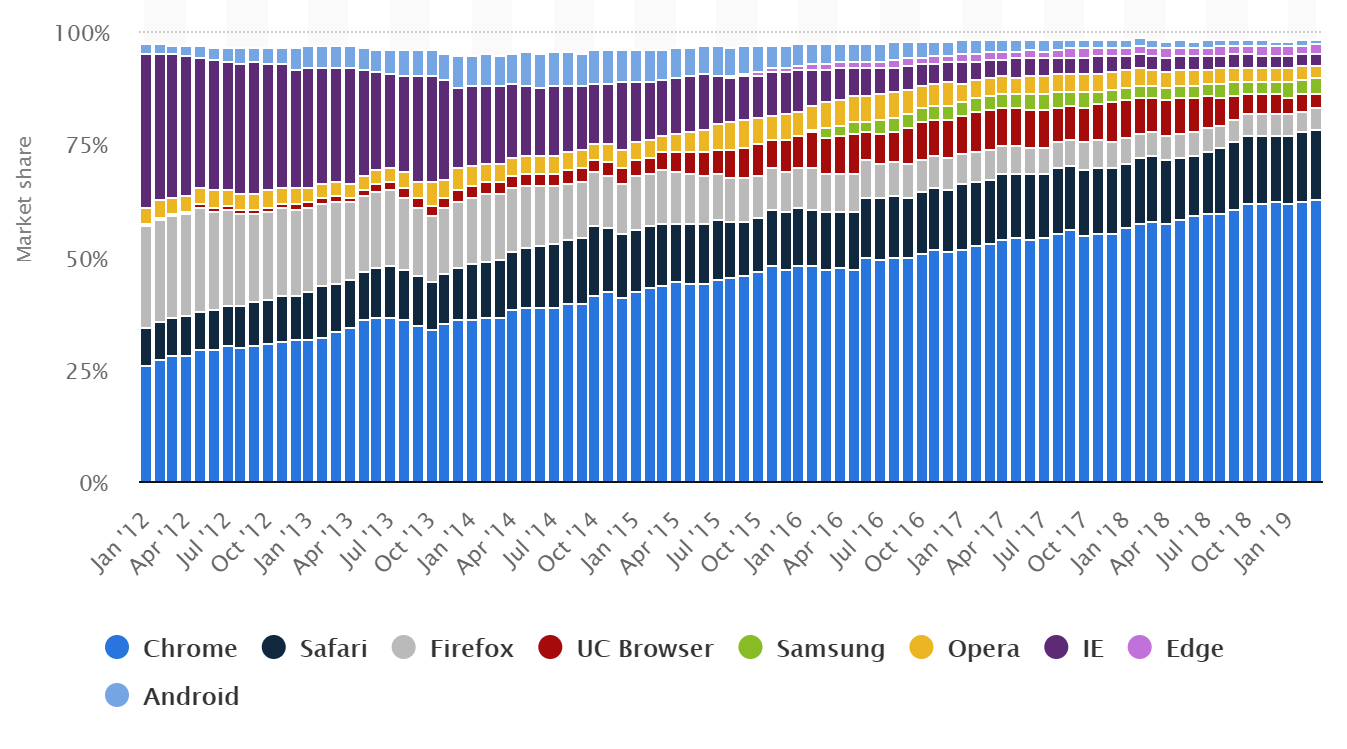
\includegraphics[width=\linewidth]{img/browser_market_share_2019.png}
  \caption[]{Global web browser market share in the 2012-2019 interval \footnotemark[5]}
  \label{fig:browser_market_share_2019}
\end{figure}

\footnotetext[5]{Image from \cite{browser_market_share_2019}}

Prateek Mehta defines Google Chrome extensions in his book \cite{creating_google_chrome_extensions} as:
\begin{displayquote}
  (\dots) browser extensions for the Google Chrome web browser.
  Browser extensions are programs that run within the context (security sandbox) of a web
  browser. They help to provide new functionality(ies) by combining existing features of the
  web browser and make it possible for users to do many things at once!
\end{displayquote}

Extensions for Google Chrome are very lightweight, being composed of just a few components written using web development technologies, such as JavaScript, HTML and CSS. These components are the background script, the popup page, which is controlled by the popup script forming the user interface of the extension, an options page, controlled by the options script and a content script. All of these components are packaged and marked in the extension's manifest file. They communicate by messages or direct connections using Google's extension API. This can be seen on a component diagram of a simple Chrome extension on figure \ref{fig:chrome_extension_component_communication}. It is worth noting that the Chrome extension API was designed to help make asynchronous extensions to enable concurrency between multiple different components of the browser \cite{chrome_extension_docs}.

\begin{figure}[ht]
  \centering
  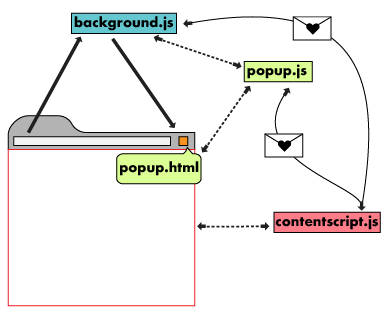
\includegraphics[width=0.5\linewidth]{img/messagingarc.png}
  \caption[]{Component diagram of a simple Google Chrome extension \footnotemark[6]}
  \label{fig:chrome_extension_component_communication}
\end{figure}

\footnotetext[6]{Image from \cite{chrome_extension_component_communication}}

The manifest file is a mandatory JSON file which contains important information about the extension, so that the browser knows how to handle it or what to display in the extensions view about it. The extension contains three mandatory fields: the manifest version, the extension name and the extension version. Google recommends you to include fields containing the extension's description, an icon set, and a default locale field which marks the subdirectory containing strings for the extension's localization. The extension's functionality scripts are marked in the \lstinline$browser_action$ or \lstinline$page_action$ field. Optionally, other fields can be added, such as the author, a version name, the permissions requested for the extension, the background script and data about it or the options page and further data about it.

The background scripts are embedded in an automatically generated html page which only contains elements with \lstinline$script$ tags which contain \lstinline$src$ tags with the relative path to the background scripts. This page is called the background page. The background scripts monitor some browser events, such as the extension being first installed or updated, a message being sent by the content script or another extension, some other view of the extension calling the background page. The background page is only loaded in the correct context and unloaded on idle. As a reaction to the events which activate the background page, the script runs some instructions. Once activated, background pages will remain active until it finishes running the response instructions.

The use interface of the extension is composed by the popup page and its controller, the popup script. The popup page is very much like a webpage: it is an HTML file, which can contain links to CSS files or sripts, but inline JavaScript is banned to increase visibility. It should be as simple as possible because the extension is meant to ease a user's interaction with the browser, not make it harder.

Content scripts are JavaScript files that run in the context of a web page and can read the contents of a webpage using the Document Object Model (DOM) of said web page, thus being able to modify it or send information to the parent extension. The content script communicates with the rest of the extension via messages.


\chapter{Detailed Design and Implementation}

\section{Conceptual Architecture}

This section presents the Conceptual Architecture of the complete system. Due to the complexity of some modules, the architecture of the modules themselves can be seen in the section describing the modules and components.

The client-server architecture is the system's foundation. The server side has multiple components: a database server, which deploys the database for the RESTful web sevice to interface with; a RESTful web server, which deploys the RESTful web service to be accessible by every other component in the system's architecture; and a web page server, which deploys the web app so that this can be accessed by the browser. The client side is formed by a web browser, preferably Google Chrome. The browser extension is loaded onto it. The browser renders the Web app to display this, creating the largest part of the user interface. The browser extension redirects its user to the web app, and checks for supported product's URLs by using some functionalities exposed by the RESTful web service. The system is also build using a layered architecture, having three layers: the front-end which is the part that the user directly interacts with, composed of the web site and the Chrome extension; the back-end which is the working mechanism of the project, composed of the RESTful web service and the scraping system; and the database, an individual layer used for data storage. Figure \ref{fig:app_conceptual_architecture_system} presents this, and it can also be seen as a deployment diagram of the system.

\begin{figure}[ht]
  \centering
  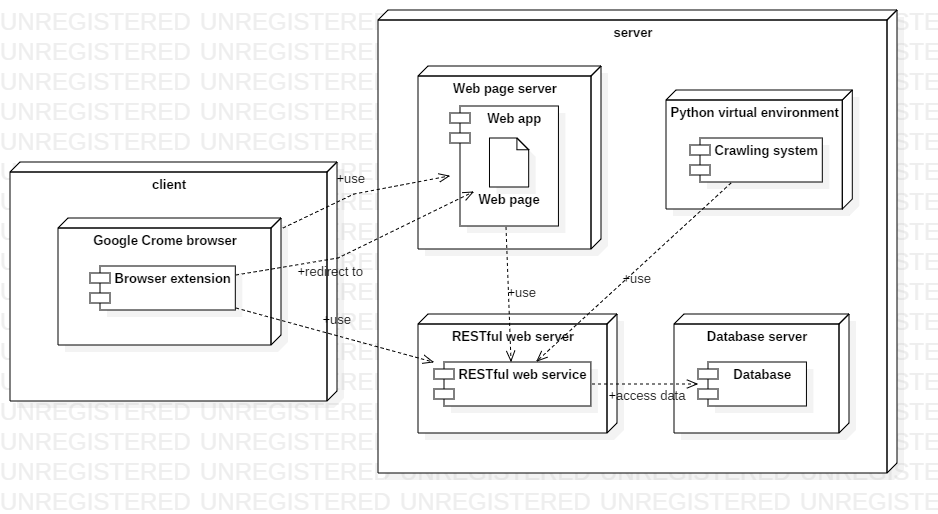
\includegraphics[width=0.65\linewidth]{img/app_conceptual_architecture_system.png}
  \caption[]{Conceptual architecture / deployment of the system}
  \label{fig:app_conceptual_architecture_system}
\end{figure}


\section{Use Cases} \label{sec:use_case}

A use case diagram presents the use cases of the application and the distinguished actors that can interact with the system. It offers a general overview for the functionalities that the system can be used for.

The application's users can be categorized into the following groups: guest, user, admin, system maintainer. The guest, user and admin interact with the application exclusively via the front-end part of it. The system maintainer interacts with the web crawling module in the back-end via a terminal. The full Use Case diagram can be seen in figure \ref{fig:app_use_case}.

A system maintainer may only interact with the application by starting a crawling process.

The admin, guest and user have three commonly accessible functionalities: using the Chrome extension, searching for a product on the webpage and looking at the details of a product they seached for.

Besides the common actions, a guest may register to get an account or log in to an account, transcending to a user.

A user can logout of their account to go back to guest level, add a product they searched for to their favourites, view the list of products they favourited or remove a product from the favourites list.

An admin may see the full list of currently available products through a special view, they can create a new empty product entry or update the data in an existing product (currently only its name). An admin may interact with a product's URLs by a separate view, adding a new URL-price matching, with an empty price element, update the URL or domain of a product's URL.

\begin{figure}[ht]
  \centering
  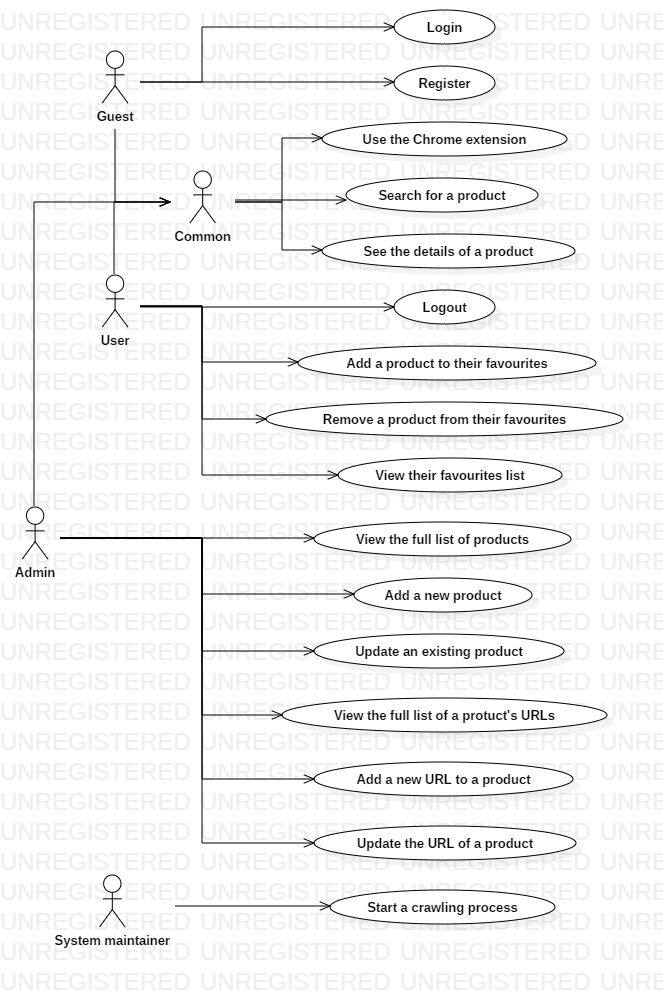
\includegraphics[width=0.5\linewidth]{img/app_use_case.png}
  \caption[]{The Use Case diagram of the application}
  \label{fig:app_use_case}
\end{figure}

Out of the listed use cases, a specific case for using the Chrome extension and for starting a crawling process has been further described in more details.


\subsection{Get the Best Offer for a Product} \label{subsec:use_case_not_cheapest}

\subsubsection{Brief Description}

The purpose of this section is to capture the flow of events that an actor must follow in order to get the best offer for the product they wish to purchase.


\subsubsection{Primary Actor}

Web customer


\subsubsection{Stakeholders and Interests}

Web customer – interested in having an accessible tool to get the best offer for the product they wish to buy


\subsubsection{Flow of Events}

The flow of events for this use case can be seen in figure \ref{fig:flow_not_cheapest_offer}.

\begin{figure}[ht]
  \centering
  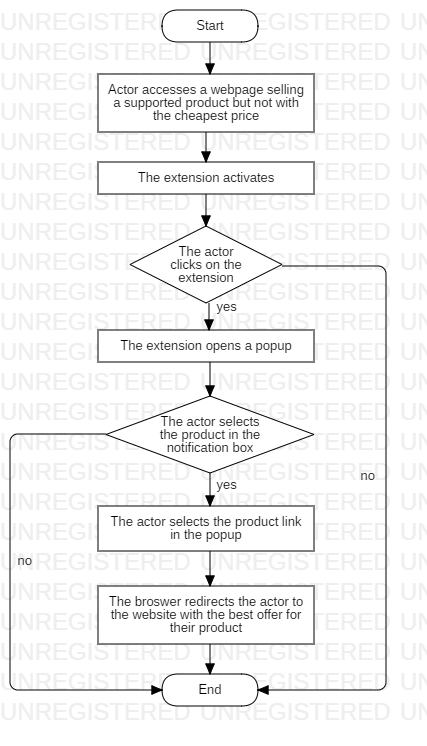
\includegraphics[width=0.4\linewidth]{img/flow_not_cheapest_offer.png}
  \caption{Flow of events when a user accesses a supported product's web page which does not sell the product at the cheapest price}
  \label{fig:flow_not_cheapest_offer}
\end{figure}


\begin{enumerate}

  \item \textbf{Main Flow}

  \begin{enumerate}
    \item \textbf{Use Case Start} - This use case starts when the actor accesses the webpage of a supported item on a supported webshop’s domain and the price is not the cheapest.
    \item The Google Chrome browser extension notices that the actor accessed a supported webpage and activates.
    \item The actor clicks on the extension. \label{step:open_extension}
    \item The extension opens a popup.
    \item The actor clicks the product link in the popup. \label{step:select_product_link}
    \item The browser redirects the actor to the website selling the same item at the cheapest price currently tracked in the system.
    \item The actor gets to the website selling the item at the lowest price.
  \end{enumerate}


  \item \textbf{Alternate Flows}

  \begin{enumerate}
    \item This flow can occur at step \ref{step:open_extension}, where the actor does not click the extension.
    \begin{enumerate}
      \item The main flow ends.
    \end{enumerate}

    \item This flow can occur at step \ref{step:select_product_link}, where the actor does not click the product link in the popup.
    \begin{enumerate}
      \item The main flow ends.
    \end{enumerate}
  \end{enumerate}

\end{enumerate}


\subsubsection{Preconditions}

\begin{enumerate}
  \item The actor has Google Chrome installed on their machine to be able to install the extension for the FEBS.
  \item The FEBS Google Chrome browser extension is installed.
\end{enumerate}


\subsubsection{Postconditions}

\begin{enumerate}
  \item The actor is on the webpage selling the product they wish to buy at the best price.
\end{enumerate}


\subsection{Update the Data Available in the Database for Items Present on a Certain Supported Domain} \label{subsec:use_case_crawl_update_database}

\subsubsection{Brief Description}

The purpose of this section is to capture the flow of events that an actor must follow in order to update the data available in the database for items present on a certain supported domain.


\subsubsection{Primary Actor}

System maintainer


\subsubsection{Stakeholders and Interests}

System maintainer – interested in having an easy to use method to keep the database up to date.


\subsubsection{Flow of Events}

The flow of events for this use case can be seen in figure \ref{fig:flow_crawl_update_database}.

\begin{figure}[ht]
  \centering
  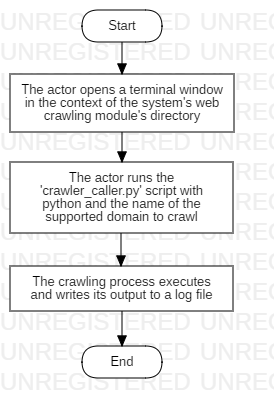
\includegraphics[width=0.4\linewidth]{img/flow_crawl_update_database.png}
  \caption{Flow of events when a system maintainer wants start a crawling process on a supported domain to update the database}
  \label{fig:flow_crawl_update_database}
\end{figure}

\begin{enumerate}

\item \textbf{Main Flow}

  \begin{enumerate}
    \item \textbf{Use Case Start} - This use case starts when the actor opens a terminal window in the context of the system's web crawling module's directory.
    \item The actor runs the \lstinline$python bachelor_project/crawler_caller.py <domain_name>$ commain, where the inputted \lstinline$domain_name$ mandatory parameter is from the list of supported domains.
    \item The crawling process automatically executes, writing its output to a log file and automatically persisting the changed items in the database using the RESTful web service.
  \end{enumerate}


  \item \textbf{Alternate Flows}

  This flow of events does not have alternate flows.

\end{enumerate}


\subsubsection{Preconditions}

\begin{enumerate}
  \item The actor's machine has Python 3 and the virtualenv tool installed.
  \item The actor has the virtual environment of the crawling module activated.
\end{enumerate}


\subsubsection{Postconditions}

\begin{enumerate}
  \item The products with changed data fields are persisted in the database.
\end{enumerate}


\section{Class Diagrams}

The appliation is very complex code-wise and is composed of many different modules, because of this, the class diagrams are described in pieces, grouped after the modules.


\subsection{RESTful Web Service Module Class Diagram}

The class diagram for the RESTful Web Service written in Java can be seen in figure \ref{fig:app_class_rest}. We can see how the module is split into two layers: the Data Access Layer (DAL) and the Business Logic Layer (BLL). The DAL is further split into the entities and repositories package. The entities are used as the base model of the application. The repositories form the connection with the database to extract data which is then mapped to the entities. The BLL is split into four packages. The package handling Data Transfer Objects (DTO) contains the DTO mappings of entities, where cyclic references are eliminated by replacing an object instance in the cycle with the ID of the object. There is a need for conversion between DTOs and entities, so a package was created which contains these classes. The 'wrappers' package contains only the IdWrapper class, which is used to receive id values from requests. The 'operations' package contains the logic of the application, written into separate classes based on the main model element they deal with. The 'controllers' package contains the REST controller definitions for the diffrenet model elements. These classes use the 'operations' package's contents to fulfill their purpose. Some connections between operations, dtos and repositories, and controllers and dtos was not presented on the diagram to reduce from the existing clutter.

\begin{figure}[ht]
  \centering
  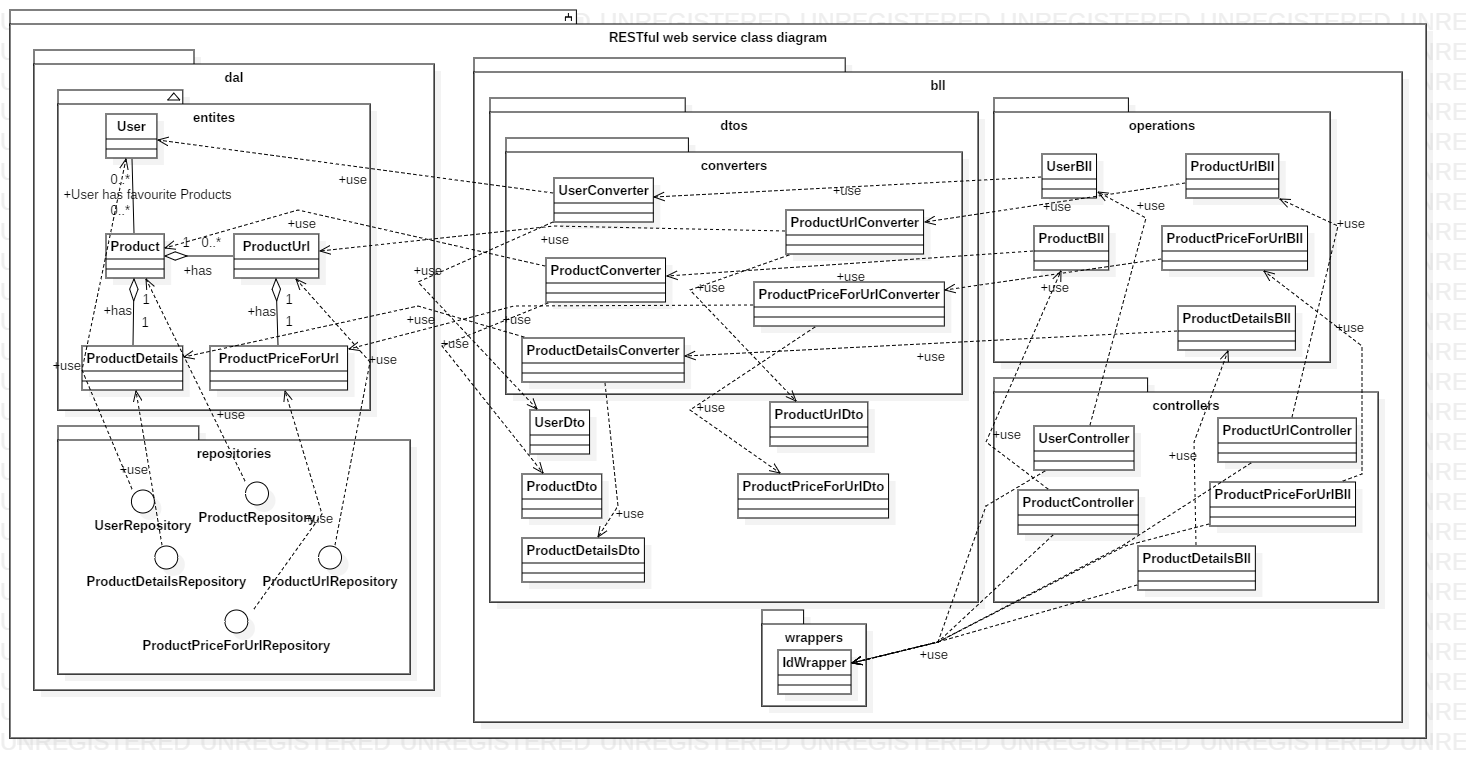
\includegraphics[width=\linewidth]{img/app_class_rest.png}
  \caption{The class diagram of the RESTful web service module}
  \label{fig:app_class_rest}
\end{figure}


\subsection{Crawling System Module Class Diagram}

The class diagram for the crawling system written with Scrapy in Python can be seen in figure \ref{fig:app_class_crawl}. We can see how the crawler caller 'sets and calls the spiders'. What actually happens here is that the crawler caller actually creates a crawling process for which the used spider is set and some parameters for the spider. The spiders then use the FillerItem class from the items.py collection to add the extracted data to, which then gets returned to the Item Pipeline, and thus to the only component active, RestPipeline, which uses the ProductLoader class to create complete product objects for the detection of database-crawl data differences. The ProductLoader class needs access to the Items defined to perform its task.

\begin{figure}[ht]
  \centering
  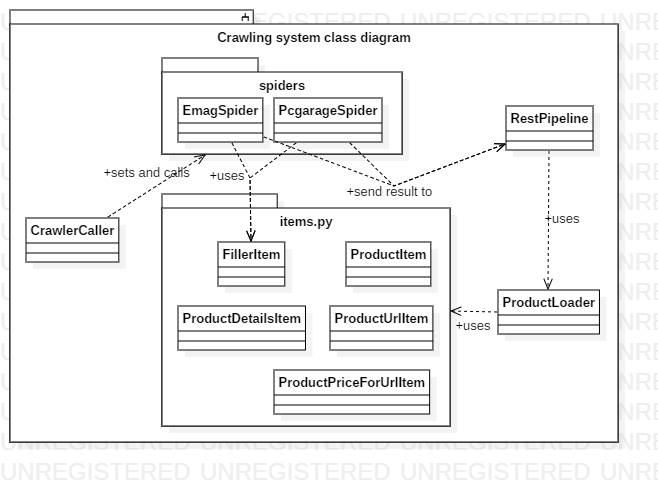
\includegraphics[width=0.6\linewidth]{img/app_class_crawl.png}
  \caption{The class diagram of the Crawling system module}
  \label{fig:app_class_crawl}
\end{figure}

\subsection{Web Site Module Class Diagram}

The class diagram of a component built with Angular can be seen in figure \ref{fig:app_class_angular_component}. The web site is built with such components. For the overall simplicity and visibility of the diagram, the components won't be presented like this, but only as a blackbox, which represents this structure. Any operation that a component does happens within its controller, the TypeScript file. 

\begin{figure}[ht]
  \centering
  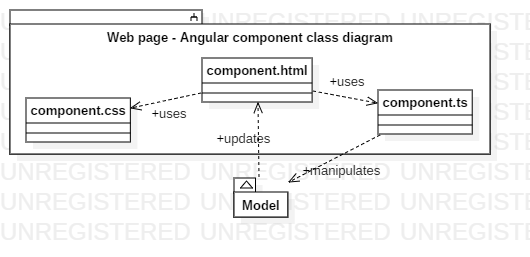
\includegraphics[width=0.6\linewidth]{img/app_class_angular_component.png}
  \caption{The class diagram of an Angular component}
  \label{fig:app_class_angular_component}
\end{figure}

The class diagram of the model built in the web site's module can be seen in figure \ref{fig:app_class_angular_model}. The web site uses elements from this model to store data and display on the views according to the Model-View-Controller architectual pattern. In the module's class diagram the model will be shown as a black box, which represents this class diagram.

\begin{figure}[ht]
  \centering
  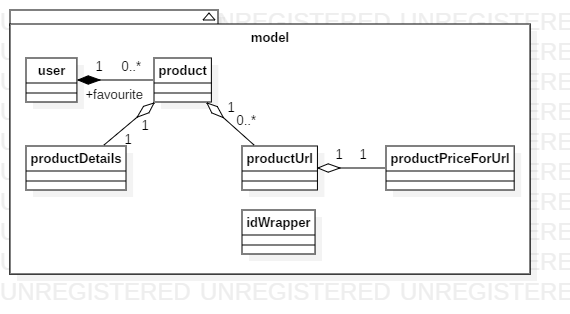
\includegraphics[width=0.6\linewidth]{img/app_class_angular_model.png}
  \caption{The model of the web site's module}
  \label{fig:app_class_angular_model}
\end{figure}

The component diagram of the web site's module can be seen in figure \ref{fig:app_class_angular_components}. The connections between the Model of the module and the rest of the components is not marked for visibility, but it there is at leas one connection between every component and the model. The Services component represents the layer which interfaces and connects to the REST API via HTTP requests and fetches or pushes data. Every other component uses at least one service from this package, but they are not marked to reduct clutter. Finally, the navigation between the pages is done using the 'AppRouting' component, which knows about every other component and knows what URL to access to get to them. Components use the AppRouting to redirect to other web pages. The 'knowledge connection' between the AppRouting component and every other component has not been shown to reduce clutter. Using these descriptions and the given diagrams, the reader should be able to imagine the class diagram of this module and see why this solution of making the diagram modular was used for better visibility.

\begin{figure}[ht]
  \centering
  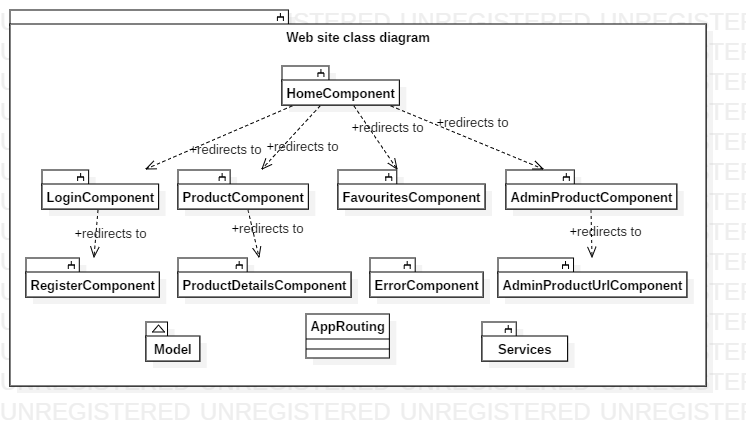
\includegraphics[width=0.75\linewidth]{img/app_class_angular_components.png}
  \caption{The diagram of the components in the web page module}
  \label{fig:app_class_angular_components}
\end{figure}


\subsection{Google Chrome Browser Extension Module Class Diagram}

The class diagram of a Google Chrome browser extension can be seen in figure \ref{fig:app_class_chrome_extension}. Here we can see how the view or the extension (popup.html) relies on its controller (popup.js) to work correctly and set it accordingly. The popup controller, in turn relies on the background script to perform its task correctly in order to have the data to do its own job.

\begin{figure}[ht]
  \centering
  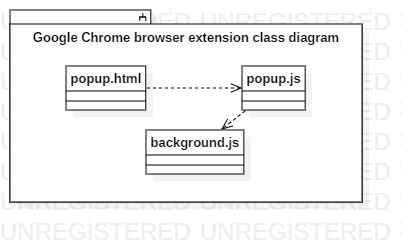
\includegraphics[width=0.5\linewidth]{img/app_class_chrome_extension.png}
  \caption{The class diagram of the Google Chrome browser extension module}
  \label{fig:app_class_chrome_extension}
\end{figure}


\section{Description of User Interaction}

In section \ref{sec:use_case}, describing the use cases of the application, there are two, more important use cases described in detail: a user getting the best offer for a product they wish to buy using the Chrome extension, and the system maintainer starting a crawling task to update the data available in the database for items present on a certain supported domain. In the following subsections I will explain and present the sequence diagrams for these use cases.


\subsection{Sequence Diagram for the Use Case 'Get the Best Offer for a Product'}

When this use case is triggered, the Chrome extension's background script gets activated via an 'onUpdated' event. When the page finishes loading the background script reads the tab's URL. The read URL's domain name is checked inside a list of supported domains with the \lstinline$checkSupportedDomain(tab)$ function. If the domain is supported, the URL is checked to be the cheapest one for a supported product with the \lstinline$checkCheaperPrice(url, tabId)$ function. This function sends an HTTP request to the REST controller dealing with ProductUrl-s, for getting the cheapest URL which is similar to the pathname of the accessed URL. The REST controller passes the argument to the method dealing with this stuff inside the BLL file which works with ProductUrl-s. The method further calls the ProductUrlRepository's custom function for finding ProductUrl-s in the database, which then retrieves all the URLs which are similar to the passed seach term (the original URL's pathname). The BLL method retrieves the first element of the passed result, in case it is not empty, goes to the URL's product and from the product's URL list it finds the URL with the cheapest price and returns it. The cheapest URL is then returned to the REST controller, which returns it as a response to the previously mentioned HTTP request. Upon receiving the response, the background script stores data about the URL (either it is not the cheapest, in which case we store the cheapest URL, or it is, in which case we only store this fact). The popup script then reads the storage content and based on what it sees it updates the view. The user then clicks on the product URL and is redirected to the cheapest URL. This can be seen in figure \ref{fig:sequence_not_cheapest_offer}.

\begin{figure}[ht]
  \centering
  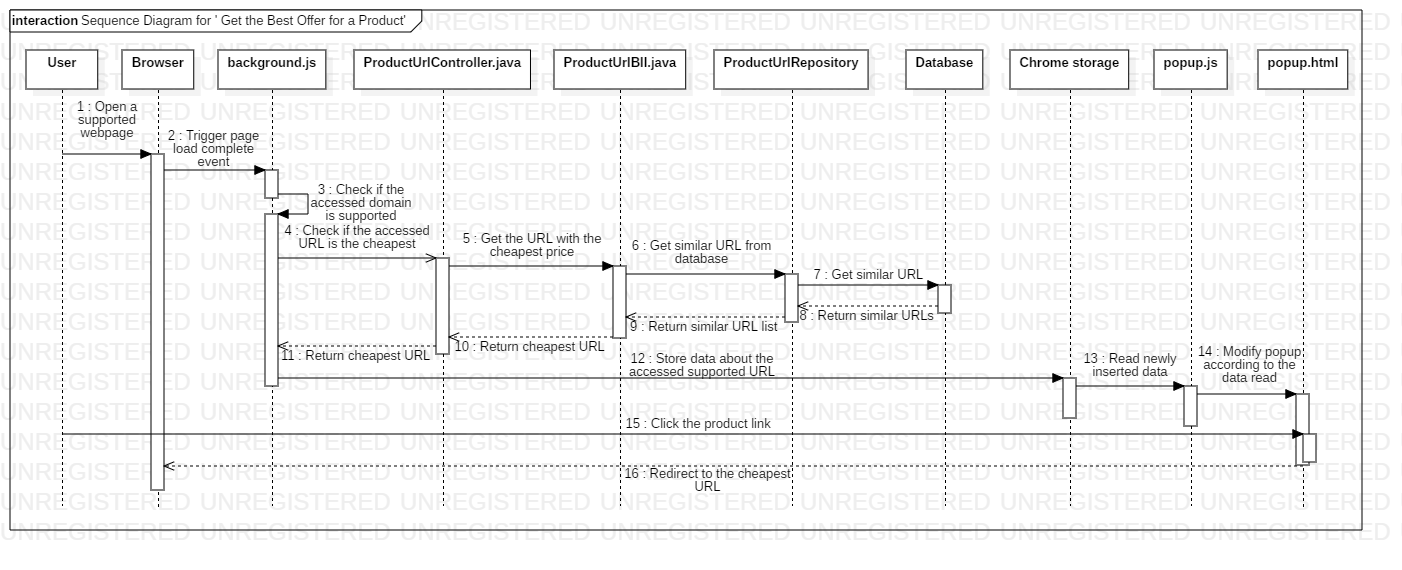
\includegraphics[width=\linewidth]{img/sequence_not_cheapest_offer.png}
  \caption{Sequence diagram of the use case found in section \ref{subsec:use_case_not_cheapest}}
  \label{fig:sequence_not_cheapest_offer}
\end{figure}


\subsection{Sequence Diagram for the Use Case 'Update the Data Available in the Database for Items Presenton a Certain Supported Domain'}

This use case is triggered by opening a terminal in the crawling module's project folder context. In the terminal the \lstinline$python crawler_caller.py <domain_name>$ command must be run, which takes one mandatory parameter containing the domain name of a supported domain. The crawling process will start from the start\_urls created by requesting the URLs belonging to this domain fom the REST controller that works with ProductUrl-s. The process of accessing a RESTful service is explained in the Sequence Diagram section for the use case in section \ref{subsec:use_case_not_cheapest}, and it can be seen in diagram \ref{fig:sequence_not_cheapest_offer}, therefore it will not be detailed again. The URLs are extracted into an array from the returned ProductUrl list, then the resulting array is set as the start\_urls parameter of the spider. Since spiders' names are the domain names they work on, the active spider is set by using the parameter passed in the terminal command. After everything is setup, the crawling process starts and executes as explained in subsubsection \ref{scrapy_arch}. It is worth noting that the spider takes the FillerItem class from the Item classes defined in the 'items.py' file, and fills it with extracted data. After the extraction is complete, the item is returned, having to pass through the Item Pipeline. In the Item Pipeline there is a component defined called 'RestPipeline'. This pipeline component first takes the product crawled from the database, then compares the data crawled to the data already in the database. If a piece of data is different, it is marked as a 'part to update'. At the end of this component, the script goes through every part to update and persists the scraped data in the database using the adequate REST controller. This can be seen in figure \ref{fig:sequence_crawl_update_database}.

\begin{figure}[ht]
  \centering
  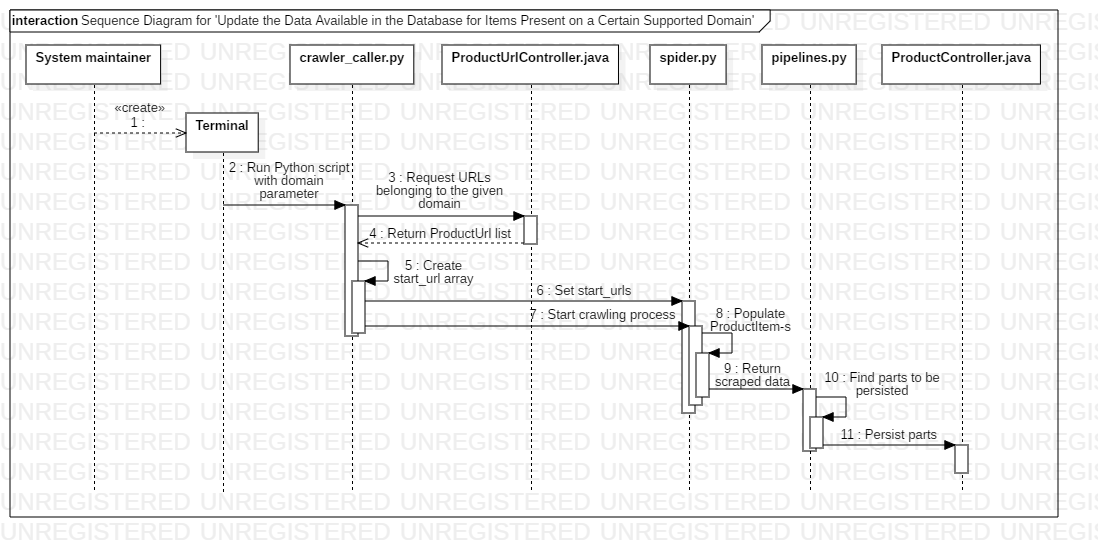
\includegraphics[width=\linewidth]{img/sequence_crawl_update_database.png}
  \caption{Sequence diagram of the use case found in section \ref{subsec:use_case_crawl_update_database}}
  \label{fig:sequence_crawl_update_database}
\end{figure}


\section{Description of impementation}

\subsection{MySQL Database}

The database is necessary for persisting the data needed to run this application. The database management system used for this application is MySQL 8.0 because of the fact that it provides a relational database and that it was familiar to use. The database schema and tables have been generated using the Spring framework's functionality, inherited from Hibernate ORM. You can see the database diagram in figure \ref{fig:database_diagram}. For the scope of this application I didn't need a database too large or too complex, and so, it consists of 5 main tables and one connection table, called user\_favourite\_products, to break the user's favourite product many-to-many connection into one-to-many connections. The main tables are the user table, storing data about the application's registered users; the product\_details table, storing specific, non-identifying, data about products; the product\_url table which contains the URLs belonging to certain products; the product\_price\_for\_url table which is in a one-to-one relation with the product\_url table, storing the price and currency that a given web page sells a product; and finally the product table, combining the tables that regard it.

\begin{figure}[ht]
  \centering
  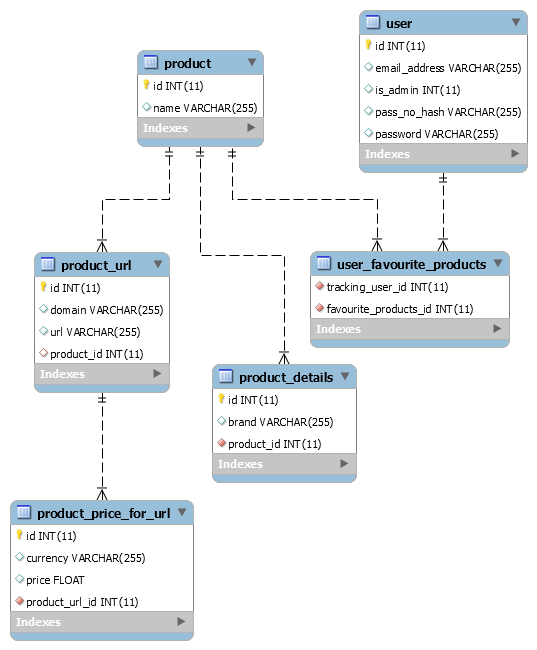
\includegraphics[width=0.65\linewidth]{img/database_diagram.png}
  \caption[]{The database diagram of the used MySQL database}
  \label{fig:database_diagram}
\end{figure}


\subsection{System Composition}

The proposed project relies on several modules for providing an accessible, easy to use tool for product price tracking. The component providing a means of communication between every other module is the RESTful Web Server that acts as a uniform means of interacting with the database of the application, as well as providing some basic functionality, such as validation of user logins. The modules being at the extremities of the system are the Web Crawling module, which contains the crawlers. The Web site is the element which provides the most functionality to the end user. The last module in the application is the Google Chrome browser extension. These modules interact to create the complete application.

The RESTful Web server connects with the database to standardize and make the connection to the database more accessible. This is done via the RESTful Web Service provided by it, which is accessible via HTTP requests to a series of URLs. The fact that HTTP is so widespread and there are ways to issue HTTP requests from almost any platform confers a very wide accessibility to it. The rest of the components connect to the web service via the exposed HTTP requests.

The crawling module connects to the web server in two points: once for requesting the URLs belonging to the domain to be crawled and then when it sends crawled data back to the web server to be peristed. The URL requesting section is done as part of the script that calls the adequate spiders based on the passed argument. Returning scraped data to the server is done in the final component of the Item Pipeline.

The web site populates its views with the data sent by the web service as a response to the web site's requests. Additionally, the web site sends data to the web service such as a user's authentication information to be validated, or updated or new data, such as a freshly registered user's data, new favourite product relations, new or updated products or product URLs.

The Google Chrome extension communicates with the web service every time a new web page is opened to check if the page belongs to a supported product. This is necessary so that the extension can constantly provide useful information to the user at a distance of a click.

This structure can be seen on figure \ref{fig:app_component_diagram}.

\begin{figure}[ht]
  \centering
  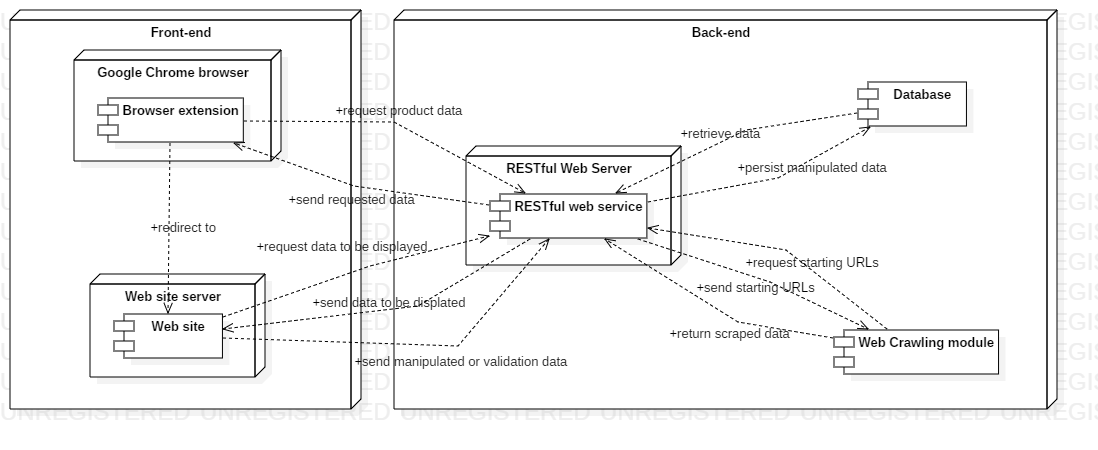
\includegraphics[width=\linewidth]{img/app_component_diagram_actual.png}
  \caption[]{Component diagram of of the proposed application}
  \label{fig:app_component_diagram}
\end{figure}


\subsubsection{RESTful Web Service Module Overview}

The web service has a layered architecture, dividing the module into two layers. The Data Access Layer, which connects to the database through the repository classes and exposes CRUD and some other functionalities. The second layer is the Business Logic Layer, which deals with implementing the methods in the Operations component which will then be exposed though the REST Controllers. The system is unable to work with pure entities, so we will need to convert them to Data Transfer Objects to eliminate cyclicity while serializing the objects returned by the methods in the Operations component. This can be seen on figure \ref{fig:app_conceptual_architecture_rest}.

\begin{figure}[ht]
  \centering
  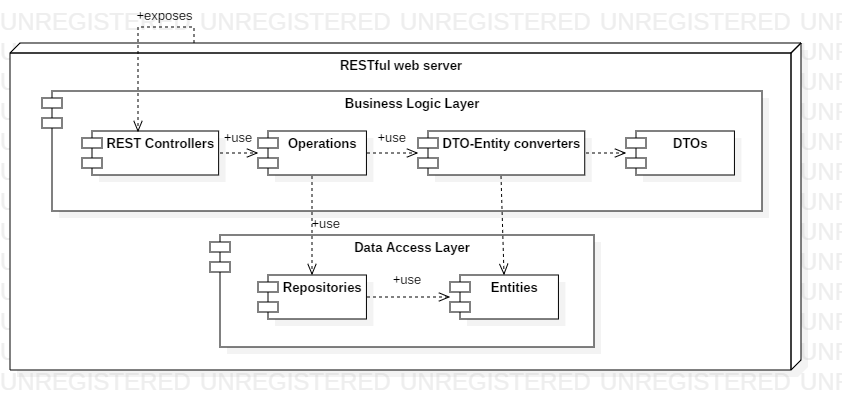
\includegraphics[width=0.65\linewidth]{img/app_conceptual_architecture_rest.png}
  \caption[]{Conceptual architecture of the RESTful web service}
  \label{fig:app_conceptual_architecture_rest}
\end{figure}


\subsubsection{Crawling System Module Overview}

The crawling system's composition has been discussed in section \ref{scrapy_arch} and can be seen in figure \ref{fig:scrapy_architecture}. The crawling module that this application uses is composed of a script that calls the crawling process and the crawling system with several subcomponents. The crawling system contains a component with spiders, the Items used by them and the components of the Item Pipeline through which the returned Items pass through. This can be seen on figure \ref{fig:app_conceptual_architecture_crawl}.

\begin{figure}[ht]
  \centering
  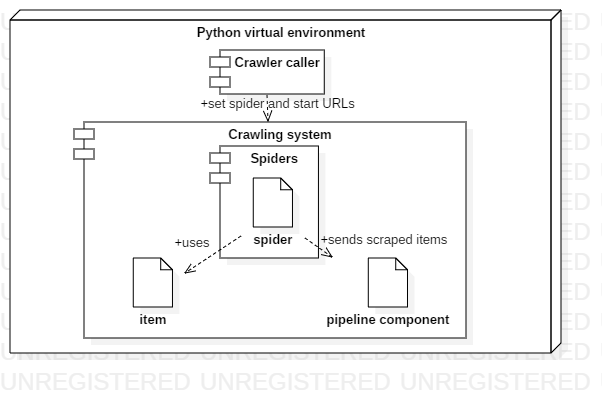
\includegraphics[width=0.65\linewidth]{img/app_conceptual_architecture_crawl.png}
  \caption[]{Conceptual architecture of the crawling system}
  \label{fig:app_conceptual_architecture_crawl}
\end{figure}


\subsubsection{Web Site Module Overview}

The web site is built using Angular, so it is sorted into components. Each component can either be a different web page or just a section of a web page. The components are built around the Model-View-Controller architecture. The components are composed of a controller script part, a view part, which is an HTML file, and a style sheet. The controller uses the model to load data with which the view is updated to show. The rest of the MVC functioning cycle is omitted from the diagram, as it is strictly limited to the architectual layout of the module. In essence, the omitted part describes the fact that the user reacts to what they see in the view by interacting with the controller functionalities linked to the view elements. The view elements take advantage of Cascading Style Sheets (CSS) to enhance their visibility and user friendliness. This can be seen on figure \ref{fig:app_conceptual_architecture_site}.

\begin{figure}[ht]
  \centering
  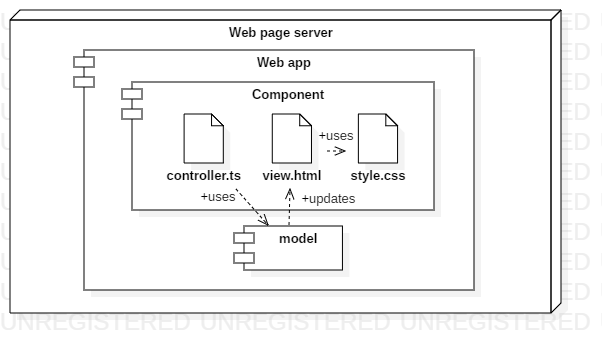
\includegraphics[width=0.65\linewidth]{img/app_conceptual_architecture_site.png}
  \caption[]{Conceptual architecture of the web site}
  \label{fig:app_conceptual_architecture_site}
\end{figure}


\subsubsection{Google Chrome Browser Extension Module Architecture Overview}

The the Google Chrome browser extension is composed of the background script, the popup script and the popul view. The background script runs when a new page is opened to get its URL, which is the checked in the database according to figure \ref{fig:app_component_diagram}. In case the URL belongs to a supported product, some data is set in the browser's storage according to the price of the product. Any time a page closes, the entry belonging to that page is eliminated from the storage. The popup script checks the content of the storage if the current tab appears as one for which it needs to display something in the view. In case this is the case, it updates the 'popup.html' file's DOM to show a specific information. This can be seen on figure \ref{fig:app_conceptual_architecture_chrome_extension}.

\begin{figure}[ht]
  \centering
  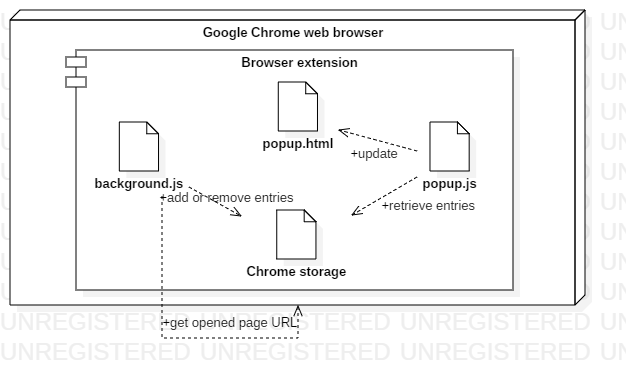
\includegraphics[width=0.65\linewidth]{img/app_conceptual_architecture_chrome_extension.png}
  \caption[]{Conceptual architecture of the Google Chrome browser extension}
  \label{fig:app_conceptual_architecture_chrome_extension}
\end{figure}


\chapter{Testing and Validation}

The application's testing was mainly done manually throughout the development period of the application. Manual testing included using different tools to check if actual results to different operation fit the expected value and by using the error and exception messages to hunt down the issues in the code. Postman was the chosen tool for testing the Spring based RESTful web service's correct functionality, as well as the exception logs outputted to the terminal in IntelliJ, the chosen Integrated Development Environment (IDE) for developing this module. Testing the web crawling module of the application was tested by taking advantage of Scrapy's schell tool and its exceptionally detailed logging, which was outputted to the terminal in PyCharm, the chosen IDE for developing this module. The Google Chrome browser was used to test the front-end functionality of the application, which includes the Angular 7 based web page and the Google Chrome browser extension. For testing the web page, the logs and error messages presented in the WebStorm IDE was also used. It is worth noting that the integrated developer tools offered by Google Chrome make debugging extensions for the browser a breeze.

Postman is a full API development environment, but for I only used it for its powerful HTTP request handling feature. Postman was used to send requests to the Spring based RESTful web service written in Java, and to validate the responses returned by it. It is worth noting that Spring makes it to that when an exception is caught during the runtime of its application, some information about it is sent through the response, thus, by using the HTTP response status, code and the information passed, then checking the full exception call stack outputted to the terminal of IntelliJ, I was able to figure out the origin of the error and fix it.

The requests used for testing the the web service's correct functionality are stored in a container called 'Collection'. For requests are further sorted into folders based on the component tested in the web service. Testing a funtionality for adding a product to the database is done by following the steps:

\begin{enumerate}
  \item Right-click the folder storing the product related requests and select 'Add Request' from the context menu.
  \item Add an adequate name for the tested request, such as 'Add product'. Optionally a description can be added.
  \item Open the created request and set its type to the one used by the web service, 'POST' in this case.
  \item Set the request's URL to the one where the resource can be found. This URL will be 'http://localhost:9906/app/product/add' in our situation.
  \item POST requests usually require a message to be passed in the request body. To set this, we need to open the 'Body' tab, select the type of the message and type in the message in the text field below. In this situation we will select the 'raw' type, with the 'JSON (application/json)' format, and writing \lstinline${"name":"Apple iPhone X"}$ for the data, as only the product name is necessary for the adding operation.
  \item Press the 'Send' button to send the request. The web service should soon send a response with a message.
\end{enumerate}

A view of the Postman window after the previous steps can be seen in figure \ref{fig:postman_add_product_example}.

\begin{figure}[ht]
  \centering
  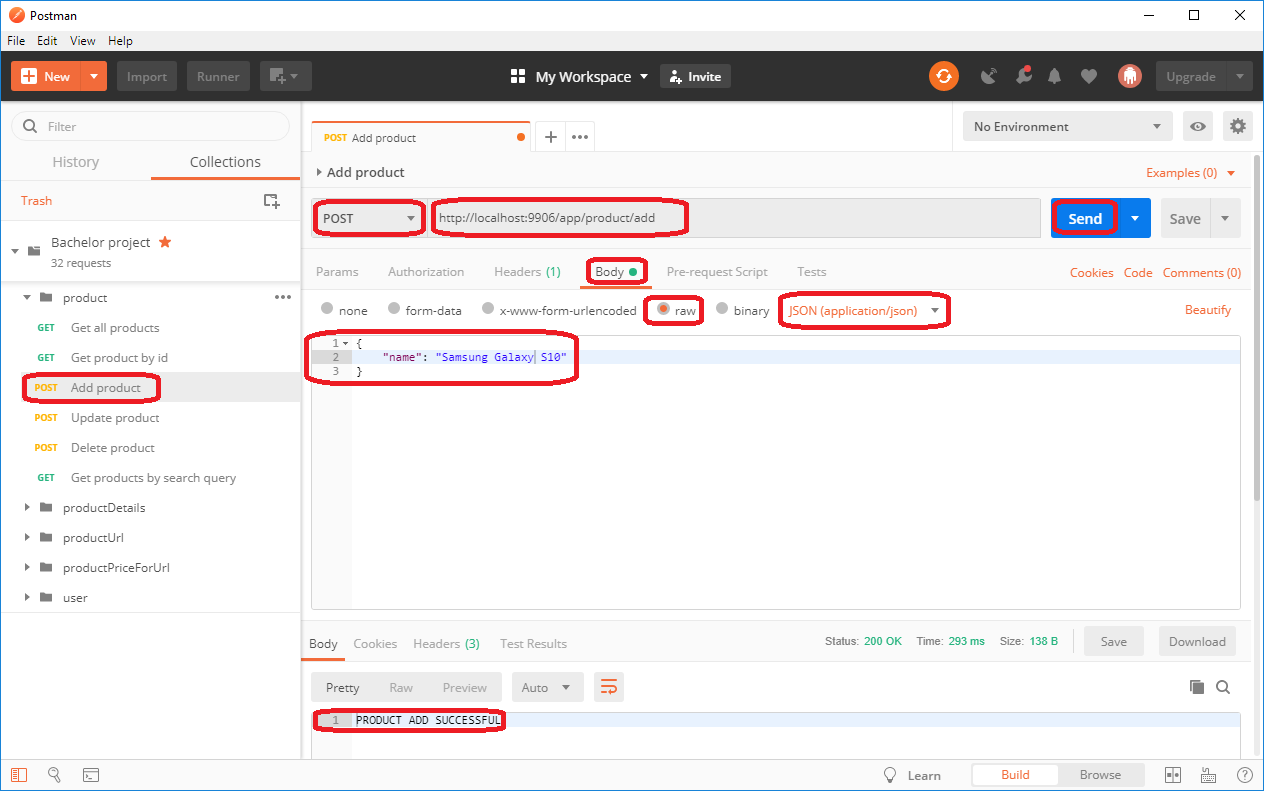
\includegraphics[width=\linewidth]{img/postman_add_product_example.png}
  \caption[]{The view of the Postman application after the steps for testing a functionality have been performed}
  \label{fig:postman_add_product_example}
\end{figure}

Testing the webcrawling module is done by opening a terminal and navigating to the Scrapy project's folder, then running the \lstinline$crawler_caller.py$ Python script, which takes one argument: the domain for which the URLs crawled should belong to. The script then connects to the web service, retrieves the URLs belonging to the given domain and passes them to the spider which works on the given domain. After this, the crawling process gets activated and the logs generated by each run of the spider are put into a temporary file at the './tmp/scrapy\_output.txt' location. These logs describe the steps through which the crawling process goes through, the data which is returned by the spider, and eventual error logs.

Testing the Google Chrome browser extension is done using the browser's developer tools. To be able to use the browser's developer tools we first need to load the extension. For this we need to go to the extensions page by either accessing the \lstinline$chrome://extensions/$ URL or by clicking the options button (three vertical dots) in the upper right corner of the browser, hovering over the 'More tools' option in the context menu, then selecting 'Extensions'. Here we need to enable developer mode by clicking on the slider in the upper right corner, then clicking the 'Load unpacked' button to finally load our extension. This process can be seen in figure \ref{fig:loading_an_extension}.

\begin{figure}[ht]
  \centering
  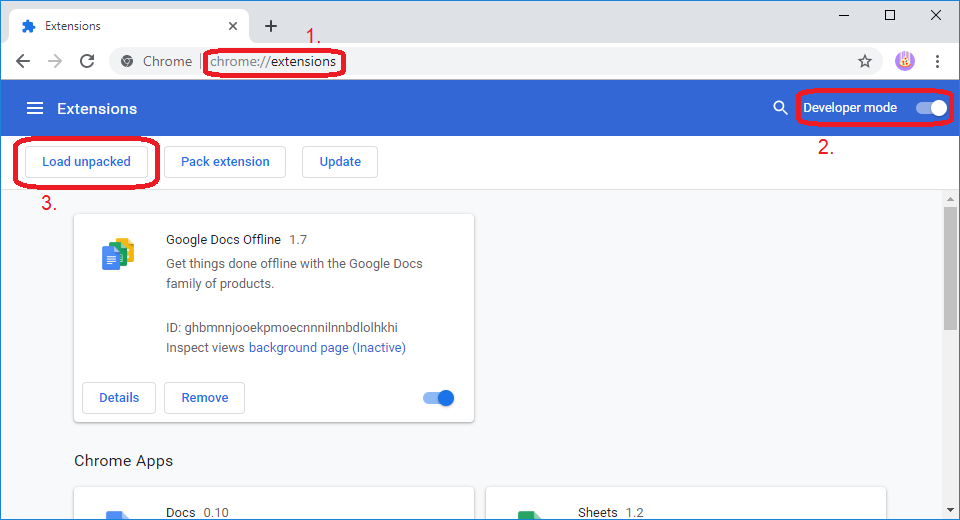
\includegraphics[width=\linewidth]{img/loading_an_extension.png}
  \caption[]{The steps required to load an extension in Google Chrome}
  \label{fig:loading_an_extension}
\end{figure}

The Google Chrome extension management system checks the loaded extension and shows a button called 'Errors' in case it detects something wrong with it. This can be seen in figure \ref{fig:extension_error}. By clicking on this button we are taken to the a page which lists every detected error, each being displayed with its error message, the context in which it is detected, the stack trace and a text box containing the context with the error containing row scrolled into view and highlighted.

\begin{figure}[ht]
  \centering
  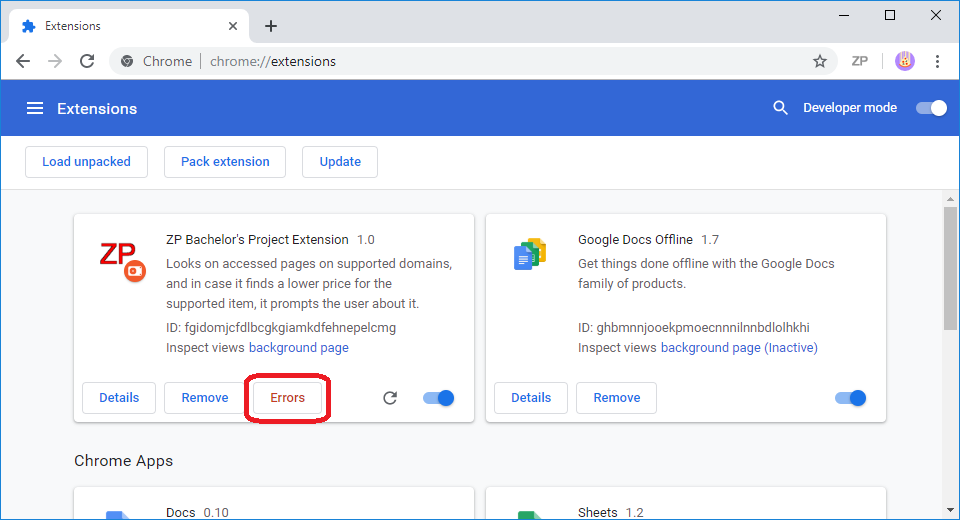
\includegraphics[width=\linewidth]{img/extension_error.png}
  \caption[]{A Google Chrome extension which contains one or more errors}
  \label{fig:extension_error}
\end{figure}

After loading the extension we can finally access the extension in the context of the developer tools. For testing the different components of the extension we have to access their developer tools in a specific way. To access the background page's developer tools we have to go to the extensions page, have developer mode active and click on the 'background page' link in the extension's section. To access the popup's developer tools we have to navigate to a page where the extension is active, then right-click the extension's icon in the taskbar, and select the 'Inspect pop-up' option. We know that the extension is active when its icon is not greyed-out. This can be seen on figure \ref{mfig:active_and_inactive_extension}

\begin{figure}[ht]
  \centering
  \begin{subfigure}{0.4\textwidth}
    \centering
    
\includegraphics[width=0.5\linewidth]{img/active_extension_icon.png}
    \caption[]{An active extension}
    \label{fig:active_extension}
  \end{subfigure}
  \begin{subfigure}{0.4\textwidth}
    \centering
    
\includegraphics[width=0.5\linewidth]{img/inactive_extension_icon.png}
    \caption[]{An inactive extension}
    \label{fig:inactive_extension}
  \end{subfigure}
  \caption{The difference between an active and an inactive extension}
  \label{mfig:active_and_inactive_extension}
\end{figure}

The developer tools in Google Chrome has several features to ease the debugging of web applications and extensions. These features include an HTML inspector, a console, a view for the sources of the analyzed component and a request tracker. The HTML inspector can be found under the 'Elements' tab in the developer tools. It is useful in finding elements in a large HTML file by clicking on something in the user interface, or the other way around, it shows which UI component does a part of HTML code describe. Showing style or the position of the element in the DOM are some other features the HTML inspector accomplishes. The console can be found under the 'Console' tab of the developer tools. It is a vital element for debugging web applications, and since every log gets outputted here it is the main tool of a developer for web debugging. The source view can be found under 'Sources in the developer tools. It encapsulates two functionalities: a source code viewer and a debugger. The debugger found within the Sources feature is extremely powerful because it includes functionalities any good debugger should have: breakpoints, a call stack viewer and a 'Watch' funtion to track the value of selected extressions/variables. The request tracker can be found under 'Network' in the developer tools. It shows a detailed list of requests made by the web page when it loads. The requests in this list have their name, status, type, initiator, size, time to complete and position in the request waterfall shown. Requests can be sorted, filtered, copied as a command in a multitude of formats, or opened to see further details, such as headers, body or preview of the body for both the request and the response. The main features used in the testing of the web page and Chrome extension of this project were the console and the debugger in the Sources feature. In figure \ref{fig:dev_tools_break} you can see a developer tools window example. You can observe the Google Chrome dev tools' structure, watched expressions, the call stack, the scope, a console with some output and the source code which has been broken into.

\begin{figure}[ht]
  \centering
  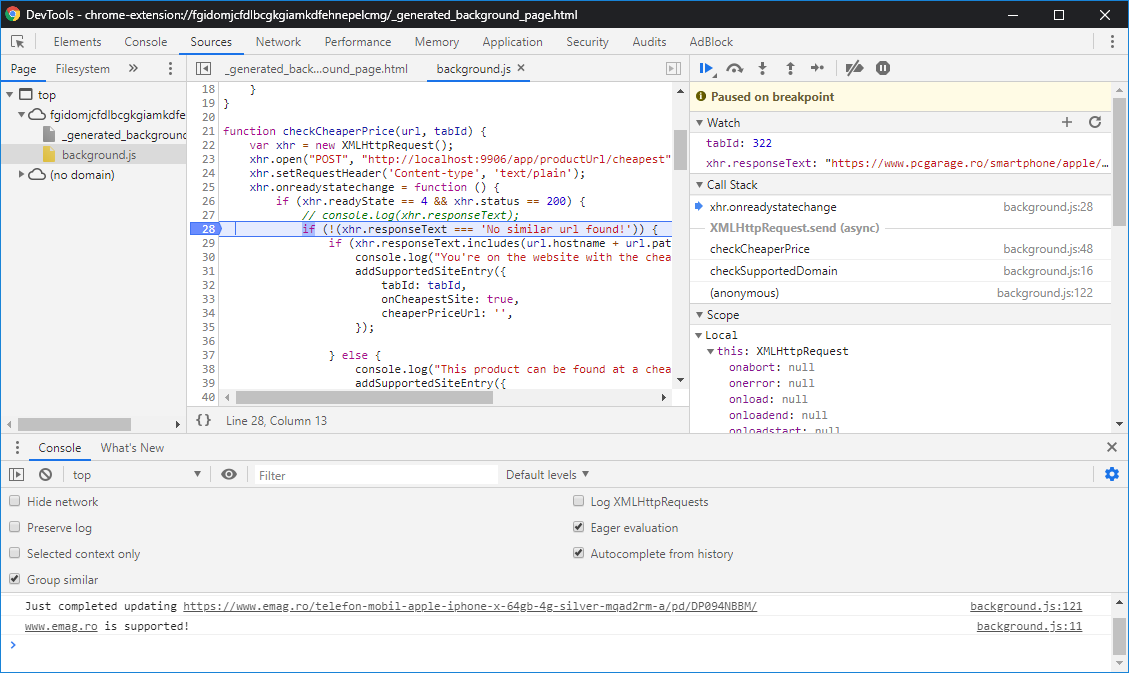
\includegraphics[width=0.97\linewidth]{img/dev_tools_break.png}
  \caption[]{A Google Chrome developer tools window}
  \label{fig:dev_tools_break}
\end{figure}

Testing the web page was done by hands-on testing the interface. As an example, at the start of the application a user might want to gain access to as many features as possible. For this they would need to register by introducing an email, a password, and repeating the password into the interface in figure \ref{fig:web_page_register}.

\begin{figure}[ht]
  \centering
  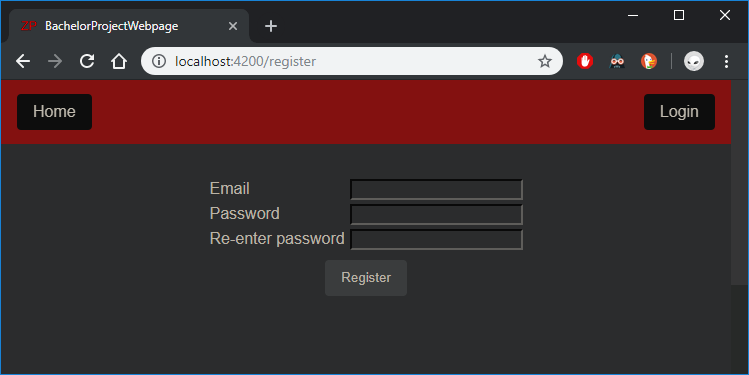
\includegraphics[width=0.85\linewidth]{img/web_page_register.png}
  \caption[]{The registration view of the application's web page}
  \label{fig:web_page_register}
\end{figure}

A test scenario for the register page would be to incorrectly repeat the password. The password fields are cleared to ease their re-inputting and the user is notified by this situation via a message appearing on the user interface stating the failure of the operation and its cause. This scenario is visible in figure \ref{fig:web_page_register_pass_mismatch}.

\begin{figure}[ht]
  \centering
  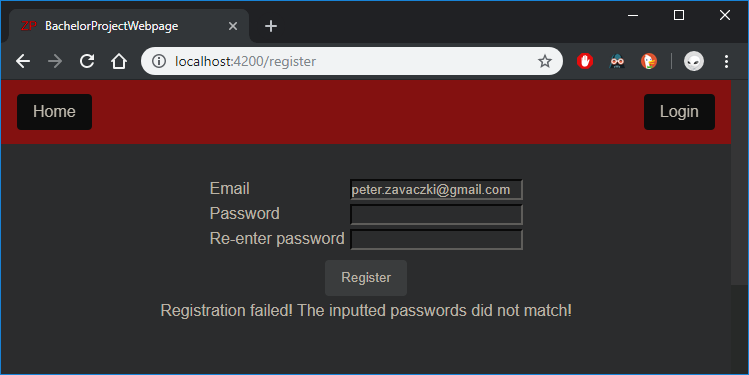
\includegraphics[width=0.85\linewidth]{img/web_page_register_pass_mismatch.png}
  \caption[]{The failure of registration due to the mismatch of the two inputted passwords}
  \label{fig:web_page_register_pass_mismatch}
\end{figure}


\chapter{User's Manual}

\section{Installation guide}

To be able to use the presented application a set of software applications must be installed on a computer. The recommended applications are MySQL Workbench 8.0 or larger, Google Chrome. For the purpose of its usage, the application will be deployed using IntelliJ, PyCharm and WebStorm from JetBrains. Additionally Java 8 or larger, Python 3.7 or larger, Node.js, Node Package Manager (npm) and Angular 7 or larger should be installed for language support.

MySQL Workbench is necessary as a database storage and handling solution for storing the data processed and manipulated by the application. MySQL can be downloaded from \url{https://dev.mysql.com/downloads/}. During the installation the user will be prompted to create a new user and a password for it. Both the username and password should be 'root'. Besides this, the installation should consist of accepting the default settings and just clicking the 'Next' button for each step of the installation. After completing the installation, the user should start the server so that the rest of the application will be able to connect to it.

A Java installer can be downloaded from \url{https://www.java.com/en/download/win10.jsp}. This installer automatically takes the last version available and installs it, thus creating a Java Runtime Environment on the computer for the application's back-end to be run in.

If the used operationg system doesn't come with Python preinstalled, it can be downloaded from \url{https://www.python.org/downloads/}. The installation is straightforward and the user should only have to click the 'Next' button until it finishes. Python is necessary for running the scraping process. After installing Python Scrapy should be installed using pip, Python's own package manager. Virtualenv is a tool used for creating independent, virtual environment for running Python scripts. It enables having different, isolated environments with different libraries and versions of libraries installed on the same machine. Installing and using virtualenv is optional, but recommended.

Node.js and npm can be downloaded from \url{https://nodejs.org/en/download/}. The installation is straightforward and the user should only have to click the 'Next' button until it finishes. Node.js is an asynchronous event driven JavaScript runtime which will serve as the running environment of our web page. Npm is Node.js' proprietary package manager. It is used to download further packages required for our web page.

Angular 7 is a JavaScript framework used for the development of the web page. It can be installed with Angular CLI through npm by running the \lstinline$npm install --save-dev @angular/cli@latest$ command line.

IntelliJ, PyCharm and WebStorm are the chosen development environments for this project. They can all be downloaded from JetBrains' website, \url{https://www.jetbrains.com/}. It is recommended that you install their professional versions. Their installation is similar and straightforward, as there should be no special input needed from the user beside clicking on the 'Next' button. After installing them, the applications components should be loaded as projects in their respective environments. After the projects are successfully loaded, the user should run the Java project from IntelliJ and the Angular based web front-end from WebStorm.

Google Chrome is the recommended browser to take advantage of the full functionality of the application, as it is the only browser for which an extension was developed. It can be downloaded from \url{https://www.google.com/chrome/}. The installation is straightforward, as there are no special steps a user needs to take. Just accept the defaults and keep clicking 'Next' until the installation finishes.

To deploy the application, first the MySQL server should be started. If you accepted the default settings during installation, it should already be running, otherwise open the MySQL Workbench and click on 'Startup / Shutdown' under the 'INSTANCE' section in the 'Navigator' toolbar, then click the 'Start Server' button. Then the applications modules should be loaded and run in their respective IDEs and projects. The \lstinline$bachelor-project-webservice$ module should be loaded in IntelliJ, the \lstinline$bachelor-project-webpage$ module should be loaded in WebStorm and the \lstinline$bachelor-project-webcrawlers$ module should be loaded in PyCharm. Loading any module in the previously mentioned IDEs is very similar, as each of those IDEs is developed by JetBrains, and each have a very similar user interface.

To load and deploy the web service module in IntelliJ follow the steps:
\begin{enumerate}
  \item Open IntelliJ and close every open project to get to the starting screen.
  \item Click the 'Import Project' button.
  \item Navigate to the location of the \lstinline$bachelor-project-webservice$ folder in the opened window, click on it, then click the 'OK' button.
  \item Select 'Import project from external model' and select 'Gradle'.
  \item In case the Gradle home is not identified, click on the option to 'Use default Gradle wrapper' and click the 'Finish' button.
  \item When prompted to overwrite the '.idea' file of the project click the 'Yes' button.
  \item To deploy the web service click on the 'Run' menu entry in the toolbar, then select the 'Run 'BachelorProjectWebserviceApplication'' option from the context menu.
\end{enumerate}

To load and deploy the web page module in WebStorm follow the steps:
\begin{enumerate}
  \item Open WebStorm and close every open project to get to the starting screen.
  \item Click the 'Open' button.
  \item Navigate to the location of the \lstinline$bachelor-project-webpage$ folder in the opened window, click on it, then click the 'OK' button.
  \item Wait until the IDE finishes indexing the project.
  \item To deploy the web page click on the 'Run' menu entry in the toolbar, then select the 'Run 'Angular CLI Server'' option from the context menu.
\end{enumerate}

To load the web crawler module in PyCharm follow the steps:
\begin{enumerate}
  \item Open PyCharm and close every open project to get to the starting screen.
  \item Click the 'Open' button.
  \item Navigate to the location of the \lstinline$bachelor-project-webcrawlers$ folder in the opened window, click on it, then click the 'OK' button.
  \item Wait until the IDE finishes indexing the project.
  \item You can start a crawling task by first entering the Scrapy project folder, by executing the \lstinline$cd bachelor_project$ command in the terminal, then running the \lstinline$python bachelor_project/crawler_caller.py <domain>$ command, where domain is a domain from the list of executed domains you wish to execute the crawling task on.
\end{enumerate}

To load the Chrome extension follow the steps:
\begin{enumerate}
  \item Opening Google Chrome.
  \item Go to the \url{chrome://extensions/} URL.
  \item Enable developer mode by clicking the slider in the upper right corner
  \item Click the 'Load unpacked' button
  \item Navigate to the location of the \lstinline$bachelor-project-chrome-extension$ folder in the opened window, click on it, then click the 'Select Folder' button.
\end{enumerate}

\section{User's guide}

The are two ways of using the application: accessing a the web page on a supported domain of a supported product and interacting with the Google Chrome extension or going to the application's main web page and interacting with that.

\subsection{Using the Google Chrome browser extension}

The user should navigate to the web page of a supported product on a supported domain. Supported domains at the time of writing are 'emag.ro' and 'pcgarage.ro' and the supported products are the 64GB version of the Apple iPhone X and the 128GB version of the Samsung Galaxy S10. For demonstration purposes, the user should navigate to \url{https://www.emag.ro/telefon-mobil-apple-iphone-x-64gb-4g-silver-mqad2rm-a/pd/DP094NBBM/}. When the extension sees that the browser entered the context of a supported domain, it activates. This can be seen by the appearance of the colored version of the extension's icon, as opposed to a greyed out one, as seen in figure \ref{mfig:users_guide_active_and_inactive_extension}.

\begin{figure}[ht]
  \centering
  \begin{subfigure}{0.4\textwidth}
    \centering
    
\includegraphics[width=0.5\linewidth]{img/active_extension_icon.png}
    \caption[]{An active extension}
    \label{fig:users_guide_active_extension}
  \end{subfigure}
  \begin{subfigure}{0.4\textwidth}
    \centering
    
\includegraphics[width=0.5\linewidth]{img/inactive_extension_icon.png}
    \caption[]{An inactive extension}
    \label{fig:users_guide_inactive_extension}
  \end{subfigure}
  \caption{The difference between an active and an inactive extension}
  \label{mfig:users_guide_active_and_inactive_extension}
\end{figure}

When the extension is active it can be clicked to open a popup. Based on the web page the user has opened, the popup can be in one of three states: if the web page is not that of a supported product; if the web page is the of a supported product but there is a cheaper alternative according to our data; if the web page is the of a supported product and this is the cheapest one, according to our data. These states can be seen on the figure \ref{mfig:extension_popup_states}.

\begin{figure}[ht]
  \centering
  \begin{subfigure}{\textwidth}
    \centering
    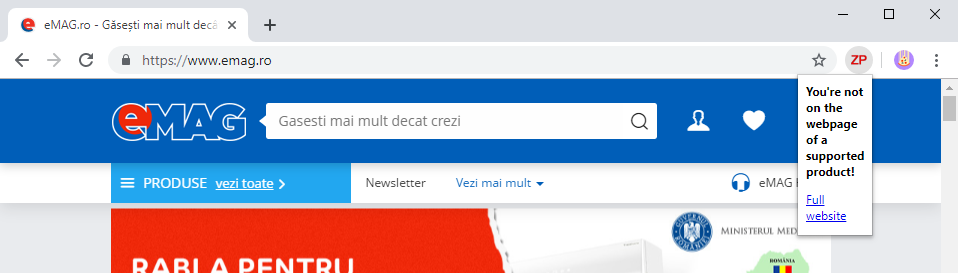
\includegraphics[width=0.8\linewidth]{img/extension_popup_not_supported.png}
    \caption[]{The extension's popup showing that the opened page does not belong to a supported product}
    \label{fig:extension_popup_not_supported}
  \end{subfigure}
  \begin{subfigure}{\textwidth}
    \centering
    
\includegraphics[width=0.8\linewidth]{img/extension_popup_cheaper.png}
    \caption[]{The popup showing that the opened page not the cheapest alternative of a supported product}
    \label{fig:extension_popup_cheaper}
  \end{subfigure}
  \begin{subfigure}{\textwidth}
    \centering
    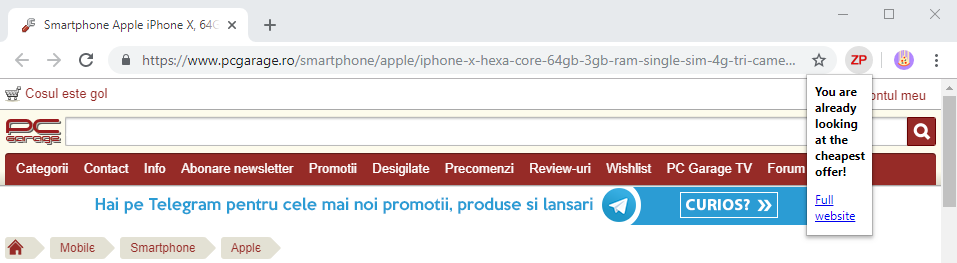
\includegraphics[width=0.8\linewidth]{img/extension_popup_cheapest.png}
    \caption[]{The popup showing that the opened page is the cheapest alternative of a supported product}
    \label{fig:extension_popup_cheapest}
  \end{subfigure}
  \caption{The extension's popup's different states based on the opened URL}
  \label{mfig:extension_popup_states}
\end{figure}

A single element is constant on the popup: the link towards the application's web page. Clicking this link will open a new tab with the home page of the application. The other elements appearing on the popup is the one that shows the status of the webpage: not a supported product, not the cheapest supported product, or cheapest supported product. There is always message showing this fact, but in the case when we are on a page with a supported product which is not the cheapest one, we can see a link to the page which sells the cheapest product. Clicking this link will open a new tab with the link selling the supported product for the cheapest price.


\subsection{Using the application's web page}

The application can be used by three types of users: guests, which are unregistered regular users, registered regular users, and registered administrators. Each of these users have different accessible functionalities. Guests may search for products based on parts of the product name, view details of products resulting from the search, register to get a regular user account, and log in to an account to get to the logged in user level. Compared to guests, logged in regular users may also add or remove products from their favourites list, thus making the tracking of certain products easier. Logged in users lose the ability to register or log into another account, a user being able to perform these actions again only after they have logged out. Administrators are basically logged in users with some additional privileges privileges. They are able to manage products, meaning that they can see every product, add new products, update existing products after selecting one from the list of current products and manage the products' URLs. Managing the product URLs means that the admins are able update an URL after they select it and to add new URLs to the product they currently manage. In turn, the admins are not able to add products to a favourites list, as this should be a useless functionality for them, they shouldn't use the app to track products.

When a user accesses the web page it is welcome by a greeting according to the user's type. This can be seen in figure \ref{mfig:web_page_home_differences}. Please note that the home page is fully visible to every kind of user as in figure \ref{fig:web_page_home_guest}, but the rest has been cut for the sake of saving space.

\begin{figure}[ht]
  \centering
  \begin{subfigure}{\textwidth}
    \centering
    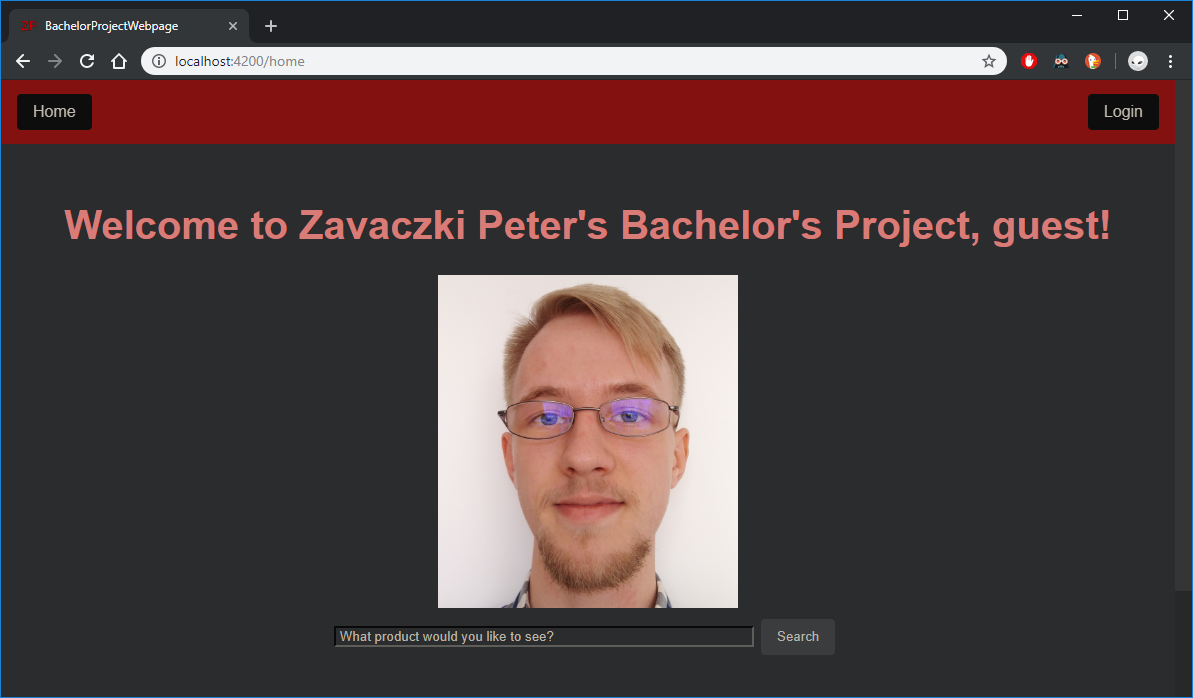
\includegraphics[width=0.75\linewidth]{img/web_page_home_guest.png}
    \caption[]{The home page, as seen by a guest}
    \label{fig:web_page_home_guest}
  \end{subfigure}
  \begin{subfigure}{\textwidth}
    \centering
    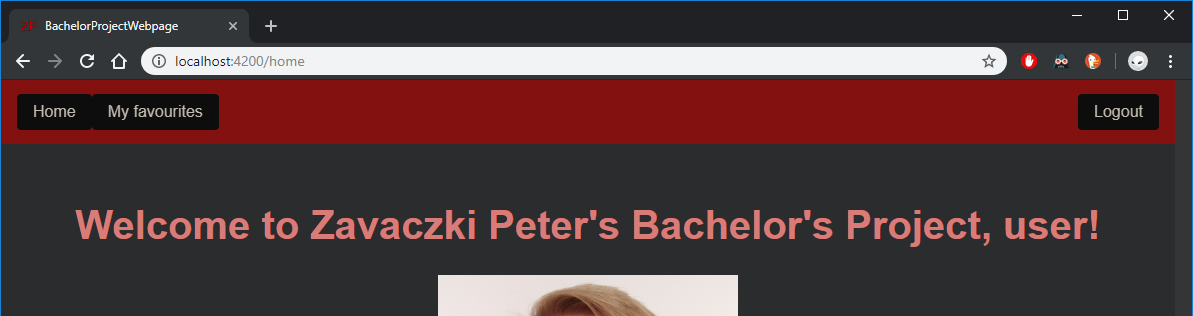
\includegraphics[width=0.75\linewidth]{img/web_page_home_user.png}
    \caption[]{The home page, as seen by a user}
    \label{fig:web_page_home_user}
  \end{subfigure}
  \begin{subfigure}{\textwidth}
    \centering
    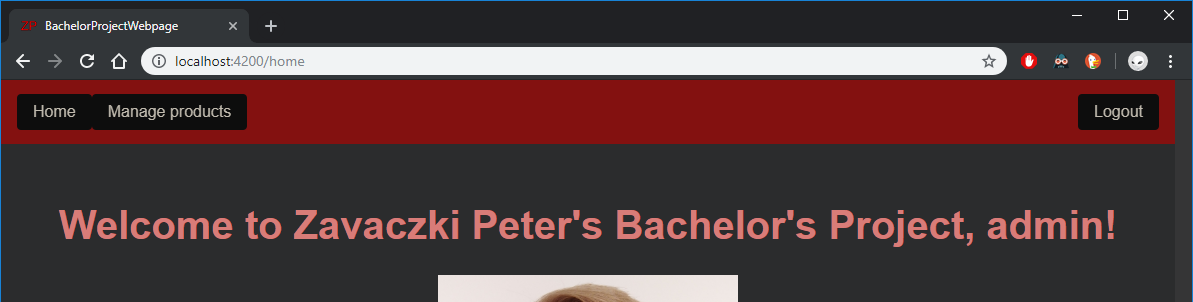
\includegraphics[width=0.75\linewidth]{img/web_page_home_admin.png}
    \caption[]{The home page, as seen by an admin}
    \label{fig:web_page_home_admin}
  \end{subfigure}
  \caption{The appearance differences of the home page based on the user's type}
  \label{mfig:web_page_home_differences}
\end{figure}

If a guest user wishes to have access to the web page they need to log in. This can be done by going to the Login page by clicking the 'Login' button in the navigation bar, anywhere the usguester might be. While on the Login page, the guest can enter an email and password combination to attempt to log in. In case any of the two are incorrect a message is shown and the data in the password field is deleted so that the inputting of a new password is easier. This can be seen in figure \ref{fig:web_page_login}. If the guest doesn't have an account, the guest can click the link in the 'You don't have an account? Register \underline{here}' section thus being redirected to the Register page.

\begin{figure}[ht]
  \centering
  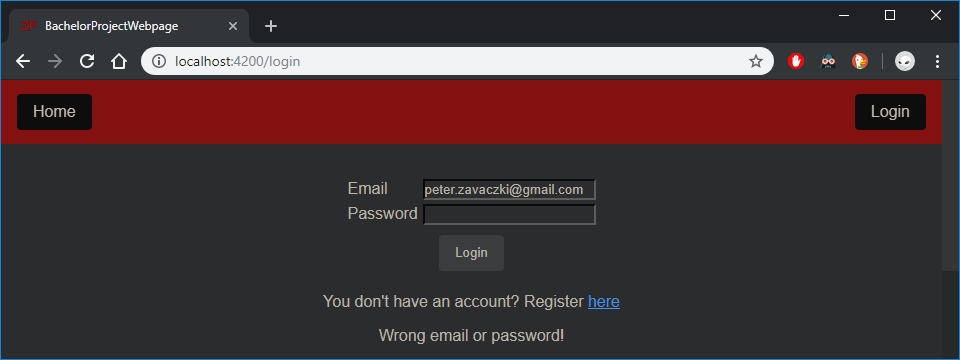
\includegraphics[width=0.75\linewidth]{img/web_page_login.png}
  \caption[]{The view shown after the guest attempts to log in with an incorrect email or password}
  \label{fig:web_page_login}
\end{figure}

To register the guest has to navigate to the Register page and input an email and a password and correctly repeat the password. In case the password was incorrectly repeated the password fields are cleared to ease their re-inputting and the guest is notified by this situation via a message appearing on the user interface stating the failure of the operation and its cause. This can be seen in figure \ref{fig:web_page_register_user_guide}. In case the registration is successful, the guest is notified via a message and told that they can use the account they created to log in.

\begin{figure}[ht]
  \centering
  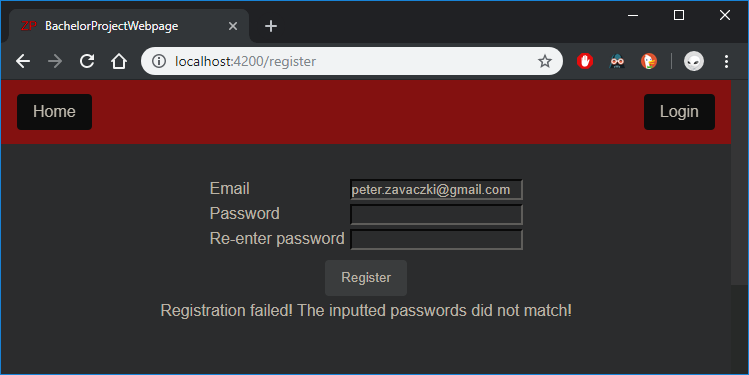
\includegraphics[width=0.75\linewidth]{img/web_page_register_pass_mismatch.png}
  \caption[]{The view shown after the guest attempts to register but is not able to successfully repeat the password}
  \label{fig:web_page_register_user_guide}
\end{figure}

Searching for a product is done by entering a search term the search bar then clicking the 'Search' button. This takes the user to the page containing a table with the products which contain the search term in their name. By clicking a row in the table of products, a 'Product Details' section opens which shows some details about the product, such as its name and its brand. Below the Product Details section there is a button called 'Open full details', which redirects to the webpage showing every relevant detail to the user, such as the product name, brand, and a table containing the URLs at which the product can be found, along with the prices at which the product is sold at that URL. If the user is logged in, a 'Favourite' button can be seen. By pressing this button the product is added to the user's favourites and a message is shown stating this fact or a message might be shown saying that the product is already in the user's favourites list. This can be seen in figure \ref{fig:web_page_product_search} and figure \ref{fig:web_page_product_details}.

\begin{figure}[ht]
  \centering
  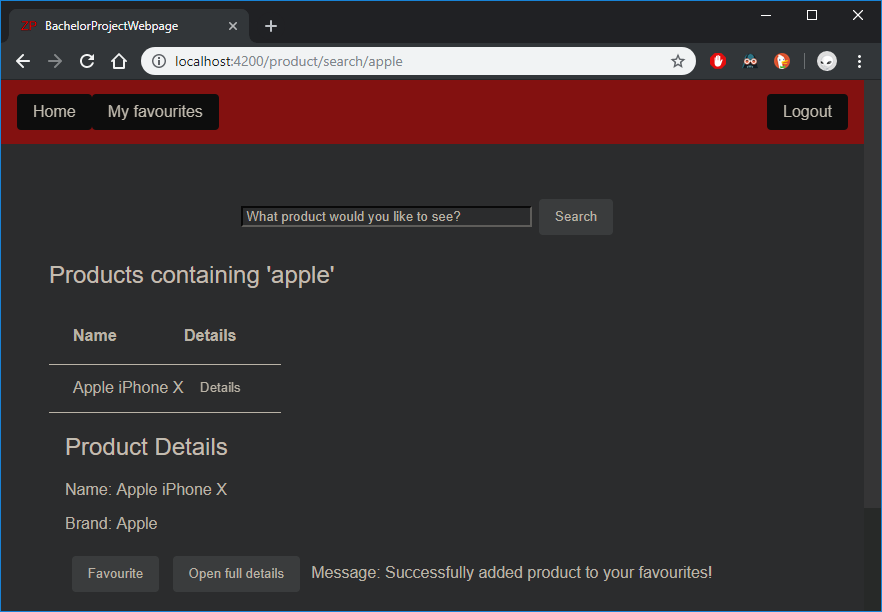
\includegraphics[width=0.75\linewidth]{img/web_page_product_search.png}
  \caption[]{The view shown after the user searches for the term 'apple', selects the first result and presses the 'Favourite' button while the product was not favourited yet}
  \label{fig:web_page_product_search}
\end{figure}

\begin{figure}[ht]
  \centering
  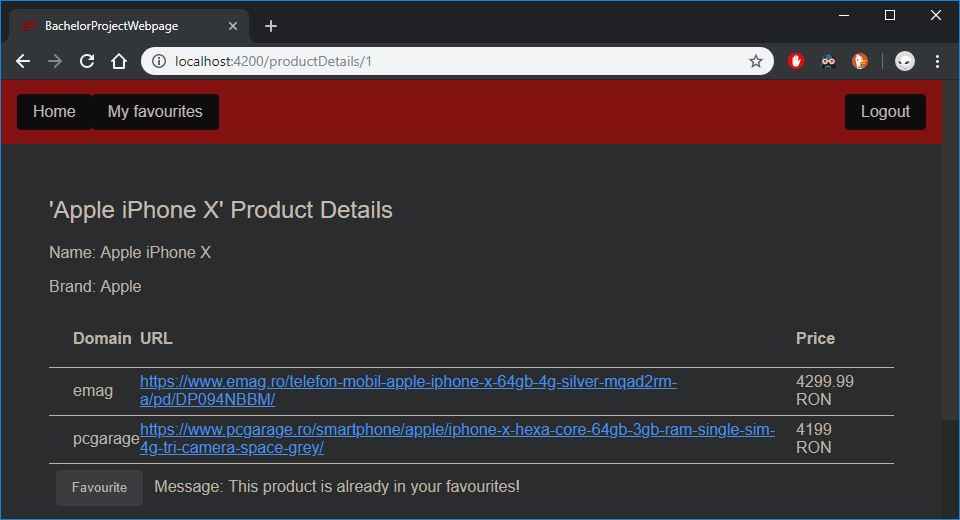
\includegraphics[width=0.75\linewidth]{img/web_page_product_details.png}
  \caption[]{The view shown after the user opens the full details page from the found product list page and presses the 'Favourite' button while the product was already favourited}
  \label{fig:web_page_product_details}
\end{figure}

The user's favourite products can be seen by clicking the 'My favourites' button in the navigation bar at the top of the page. This page has a similar functionality to the page which lists the products found after the search, except for the fact that instead of the 'Favourite' button, there is an 'Un-favourite' button which, when pressed, eliminates the product from the user's favourites list. This can be seen in figure \ref{fig:web_page_favourites} In case the user has no products in their favourites list, a message is shown stating 'No product found!'.

\begin{figure}[ht]
  \centering
  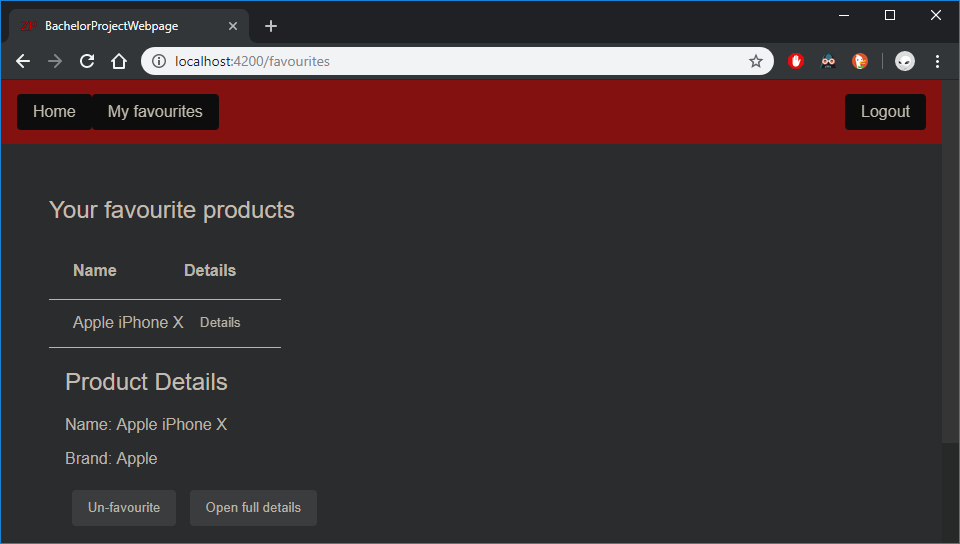
\includegraphics[width=0.75\linewidth]{img/web_page_favourites.png}
  \caption[]{The view shown when the 'My favourites' is opened and the user has a product in their favourites list}
  \label{fig:web_page_favourites}
\end{figure}

An admin can manage the products by clicking on the 'Manage products' button in the navbar. They will be redirected to a page showing every existing product in a table. Below the table there is a 'Product Details' section with an input box with the product name and, in case the admin selected a product from the table, the rest of the details of the product. An admin can add a new product by typing the name of the product they wish to add in the input box and clicking the 'Add' button. If the operation executes successfully, a message stating this fact is displayed. If the admin wishes to update a product, they have to select one from the table, edit their name and press the 'Update' button. If everything executes successfully, a message stating this fact is displayed. An 'Open full details' button is visible if the admin selected a product from the table. It works exactly like the Open full details button from the previously described searched products page. A 'Refresh list' button can be seen, which sends a new request to the web service and retrieves the current list of products, as it can be found in the database. In case the admin selected a product from the table, a 'Manage the URLs' button appears which, if clicked, takes the admin to the product URL management page of the selected product. The described admin products page can be seen in figure \ref{fig:web_page_admin_products}.

\begin{figure}[ht]
  \centering
  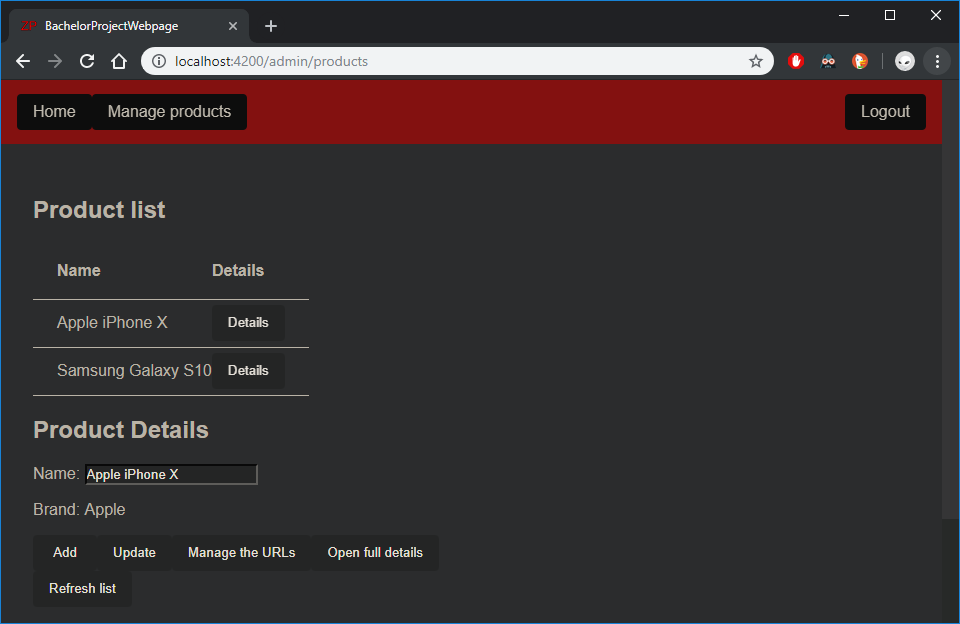
\includegraphics[width=0.75\linewidth]{img/web_page_admin_products.png}
  \caption[]{The view shown when an admin navigates to the Admin products page and selects a product from the table}
  \label{fig:web_page_admin_products}
\end{figure}

The admin product URL management page is almost identical to the admin product management page. The main difference is that there are two text fields: one for the URL and one for the domain. The page works with product URLs and these are the only fields that the admin is allowed to interact with either if he wishes to add a product URL or update one. Another change is that there is no 'Open full details' button, because every detail of the selected URL is exposed in the previously mentioned text fields. The final change is that there is no 'Manage the URLs' or similar button, as there is no composite component of the Product URLs which should be manipulated by a human agent. The described page can be seen in \ref{fig:web_page_admin_product_urls}.

\begin{figure}[ht]
  \centering
  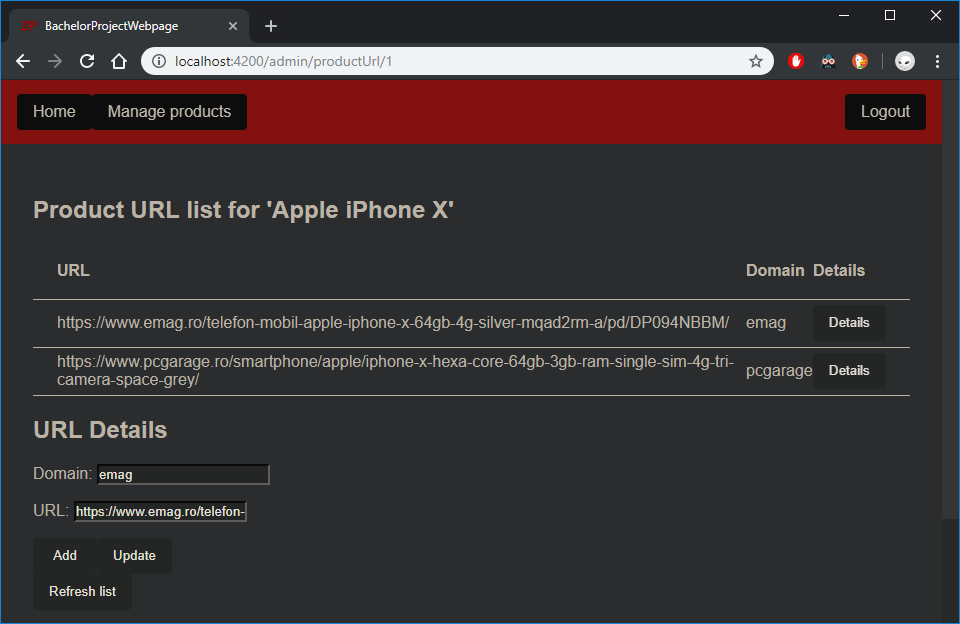
\includegraphics[width=0.75\linewidth]{img/web_page_admin_product_urls.png}
  \caption[]{The view shown when an admin chooses to manage the URLs of a selected product in the product management page and selects a product URL from the table}
  \label{fig:web_page_admin_product_urls}
\end{figure}


\chapter{Conclusions}

In the world dominated by information, options and opportunities the modern man's life is eased and made more difficult by online shopping. This aspect of life has presented companies like 'Online Comparison Shopping', who own compari.ro to create tools to keep track of the different offers across the internet.

The solution presented by compari.ro is great, but not the most accessible one, as a user would need to find its web site, navigate to it, find a product and only then could they choose a webshop to buy it from.

I have developed a web application that tracks the prices of some products across ecommerce stores and exposes this information to users through a handy Google Chrome browser extension and a web site. The goals of this application were:

\begin{enumerate}
  \item accessibility
  \item ease of use
  \item intuitiveness
\end{enumerate}

The browser extension gave the means to achieve the goal of being easily accessible. The minimal interface granted ease of use and intuitiveness to the application. Thus every proposed goal has been achieved.

On top of the proposed goal, a very maintainable core element has been created through the use of Scrapy and with the help of its components, such as the spiders or the Item Pipeline.

The application could further be developed by adding the following to it:

\begin{itemize}
  \item A large number of products with the respective URLs to increase market coverage
  \item A solution to have the web service and the web site permanently deployed
  \item Component optimization for further boosting performance, stability and maintainability
  \item A prettier user interface
  \item A solution to have the web service and the web site publicly available from the internet
  \item More scraping spiders to increase the number of domains supported and the market coverage
  \item An automated process for scraping so that the database can remain up to date without the need of a human agent
  \item A port of the extension to other significant browsers such as Mozilla Firefox
  \item A mobile application for being able to access the service on the go
\end{itemize}



%\addcontentsline {toc}{chapter}{Bibliography}
\bibliographystyle{IEEEtran}
\bibliography{thesis}%same file name as for .bib

% \appendix
\chapter{Relevant code}


\chapter{Other relevant information (demonstrations, etc.)}


\chapter{Published papers}

\end{document}
